%input macros (i.e. write your own macros file called MacroFile1.tex)
%\newcommand{\PdfPsText}[2]{
  \ifpdf
     #1
  \else
     #2
  \fi
}

\newcommand{\IncludeGraphicsH}[3]{
  \PdfPsText{\includegraphics[height=#2]{#1}}{\includegraphics[bb = #3, height=#2]{#1}}
}

\newcommand{\IncludeGraphicsW}[3]{
  \PdfPsText{\includegraphics[width=#2]{#1}}{\includegraphics[bb = #3, width=#2]{#1}}
}

\newcommand{\InsertFig}[3]{
  \begin{figure}[!htbp]
    \begin{center}
      \leavevmode
      #1
      \caption{#2}
      \label{#3}
    \end{center}
  \end{figure}
}


%%% Local Variables: 
%%% mode: latex
%%% TeX-master: "~/Documents/LaTeX/CUEDThesisPSnPDF/thesis"
%%% End: 

\documentclass[oneside,11pt]{classes/CUEDthesisPSnPDF}
% THIS IS THE MAIN FILE.
% It is dependent on the folder structure provided to you.

\title{Automatic Test Grader Using Image Processing And Machine Learning Techniques}

  \author{Andries Petrus Smit\linebreak 18183085}
  \collegeordept{\href{http://www.ie.sun.ac.za}{Department of Electrical and Electronic Engineering}}
  \university{\href{http://www.sun.ac.za}{University of Stellenbosch}}
% insert below the file name that contains the crest in-place of 'UnivShield'
  \crest{\includegraphics[width=30mm]{USwapencrestalone}}

% insert below the file name that contains the crest in-place of 'UnivShield'
% \crest{\IncludeGraphicsW{UnivShield}{40mm}{14 14 73 81}}
%
%\renewcommand{\submittedtext}{change the default text here if needed}
\degree{B.Eng Electrical and Electronic}
\promotor{Study leader: JA du Preez}
\degreedate{December 2017}

% turn of those nasty overfull and underfull hboxes
\hbadness=10000
\hfuzz=50pt

% Put all the style files you want in the directory StyleFiles and usepackage like this:
%\usepackage{StyleFiles/watermark}
\usepackage{verbatim, fixltx2e, xspace}
\usepackage{nomencl}
\usepackage{makeidx}
\usepackage{graphicx}
\usepackage{pgfplots}
\usepackage{longtable}
\usepackage{amssymb, amsmath}
\usepackage{algorithm}
\usepackage{algpseudocode}
\usepackage{multirow}
\usepackage{rotating}
\usepackage{float}
\usepackage{subfig}
%% The amsthm package provides extended theorem environments
%% \usepackage{amsthm}
\usepackage{StyleFiles/mcode}
\usepackage{algorithm}
\usepackage{algpseudocode}
\usepackage{booktabs}
\usepackage{tikz}
\usepackage{morefloats}
\usepackage[section] {placeins}
\usepackage{hyperref}
\usepackage{url}
\usetikzlibrary{arrows,positioning,fit,patterns,plotmarks}

% You may ignore these commands, but do not delete them
\newenvironment{dedication}
{
   \cleardoublepage
   \thispagestyle{plain}
   \vspace*{\stretch{1}}
   \hfill\begin{minipage}[t]{0.8\textwidth}
   \raggedright
}%
{
   \end{minipage}
   \vspace*{\stretch{3}}
   \clearpage
}

\usetikzlibrary{patterns}
\lstset{language=Matlab}
\usetikzlibrary{arrows,positioning,fit}

\newcommand{\uvec}{\mathbf{u}}
\newcommand{\vvec}{\mathbf{v}}
\newcommand{\tab}{\hspace*{2em}}
\newcommand{\halftab}{\hspace*{1em}}
\newcommand{\Naso}{Na\textsubscript{2}SO\textsubscript{4}\xspace}

%If you want to compile only a specific chapter, use this. It saves time when your document becomes %large.
%\includeonly{Chapter2/chapter2}
%\includeonly{Chapter1/chapter1}

%Hierdie command bou die Nomenclature. Die naam "skripsie" moet verander as jou hoofdokument se naam verander, bv "MarykeSkripsie.tex".
\immediate\write18{makeindex skripsie.nlo -s nomencl.ist -o skripsie.nls}
\makenomenclature



\begin{document}

%\renewcommand{\nomname}{Glossary}\check{}
%\renewcommand{\nomentryend}{.}
\renewcommand{\nompreamble}{\markboth{Nomenclature}{Nomenclature}}

\renewcommand\baselinestretch{1.2}
\baselineskip=18pt plus1pt

% Using the watermark package which is in StyleFiles/
% and to remove DRAFT COPY ONLY appearing on the top of all pages comment out below line
%\watermark{DRAFT COPY ONLY}

\maketitle

%set the number of sectioning levels that get number and appear in the contents
\setcounter{secnumdepth}{3}
\setcounter{tocdepth}{3}

\frontmatter

% Chapters will be included in this order:
%----------------------------------------

%\begin{dedication}
%Dedicated to (If you don't want to, comment this section out).
%\end{dedication}

%\addcontentsline{toc}{chapter}{Acknowledgement}
% Thesis Acknowledgements ------------------------------------------------


%\begin{acknowledgementslong} %uncommenting this line, gives a different acknowledgements heading
\begin{acknowledgements}      %this creates the heading for the acknowlegments
I would like to acknowledge my study leader, J.A. du Preez, parents and the engineering class of 2017 for their kind contribution to this project. I would especially like to give thanks to the Applied Mathematics Department of Stellenbosch University for providing the opportunity and data needed to complete this project.
\end{acknowledgements}
%\end{acknowledgmentslong}

\include{Declaration/declaration}
\addcontentsline{toc}{chapter}{ECSA Outcomes Reference}
% Thesis Acknowledgements ------------------------------------------------


%\begin{acknowledgementslong} %uncommenting this line, gives a dif{f}erent acknowledgements heading
Check of dit reg is??
\begin{ecsa}      %this creates the heading for the acknowlegments

% Table generated by Excel2LaTeX from sheet 'Sheet1'

\begin{tabular}{|p{8.3cm}|p{2.7cm}|p{1.5cm}|}
\hline
\textbf{Outcome}&\multicolumn{2}{|l|}{\textbf{Reference}}\\
\hline
& Sections & Pages\\
\hline
1. Problem solving: Demonstrate competence to identify, assess, formulate and solve convergent and divergent engineering problems creatively and innovatively. & \textit{All} & \textit{All}\\
\hline
5. Engineering methods, skills and tools, including information technology: Demonstrate competence to use appropriate engineering methods, skills and tools, including those based on information technology. & \textit{2, 3, 4, 5, 6 \& 7} & \textit{10 -- 62}\\
\hline
6. Professional and technical communication: Demonstrate competence to communicate ef{f}ectively, both orally and in writing, with engineering audiences and the community at large. & \textit{All} & \textit{All}\\
\hline
9. Independent learning ability: Demonstrate competence to engage in independent learning through well developed learning skills. & \textit{2, 3, 4 \& 5} &  \textit{10 -- 37}     \\
\hline
10. Engineering professionalism: Demonstrate critical awareness of the need to act professionally and ethically and to exercise judgment and take responsibility within own limits of competence. &\textit{8.3 \& 8.4}  &  \textit{66 -- 67}        \\
\hline
\end{tabular}





\end{ecsa}
%\end{acknowledgmentslong}

% ------------------------------------------------------------------------

%%% Local Variables:
%%% mode: latex
%%% TeX-master: "../thesis"
%%% End:


\addcontentsline{toc}{chapter}{Abstract}

% Thesis Abstract -----------------------------------------------------


%\begin{abstractslong}    %uncommenting this line, gives a different abstract heading
\begin{abstracts}        %this creates the heading for the abstract page
\nomenclature[A]{$OMR$}{Optical mark recognition}
\nomenclature[pgmAcronym]{$PGM$}{Probabilistic graphical model}
\nomenclature[A]{$NN$}{Neural network}
The aim of this research project is to develop software that can automatically grade tests, written by students on a special template. This template allows the software to extract the students' intended answers, after it has been scanned into a digital form. The standard method used in these Optical Mark Recognition (OMR) software, is to allow a learner to specify answers by colouring in bubble grids. To correct a mistake, the previous answer bubbles must first be erased and new ones coloured in. This takes time and increases the probability that a learner might colour in bubbles incorrectly. 

This research project tries to solve this problem by implementing additional software that eases the use of such a template. Using computer vision and two machine learning techniques, namely Neural Networks (NN) and Probabilistic Graphical Models (PGM), a student can now answer questions using characters and bubbles. In the case of a student number the student does not need to colour in the bubbles at all. The software implemented in this project allows for a decreased in time filling in templates like these, which decreases the number of mistakes made. Thus methods proposed here can simplifies the incorporation of OMR templates into the traditional education system.
\end{abstracts}
%\end{abstractlongs}

\addcontentsline{toc}{chapter}{Opsomming}
\include{Abstract/opsomming}

\tableofcontents
\listoffigures
\addcontentsline{toc}{chapter}{List of Figures}
\listoftables
\addcontentsline{toc}{chapter}{List of Tables}
\printnomenclature[5cm]
\addcontentsline{toc}{chapter}{Nomenclature}
\mainmatter
%\onehalfspacing

%\printnomenclature  %% Print the nomenclature
%\printglossary

% The chapters will be included in this order, and also numbered 1, 2, 3, 4,, 5, 6, 7. The file name % does not matter. I suggest you give your chapters names like "LitStudy", "Analysis", "Results" etc. If your study leader suggests a different order then it is easier to relate to the new order. The order  below is confusing, but it will still work.
\chapter{Introduction}
\label{ch:Introduction}
\graphicspath{{Chapter1/Chapter1Figures/}}
As modern technology and machine learning techniques advances, it is important for the educational sector to also continuously advance their learning environment. This allows for an ever improving learning experience in and outside the classroom. 

\section{Problem background}

\textsl{In the recent years the Applied Mathematics Department of Stellenbosch Engineering, started observing a decrease of accuracy in grading of tutorial tests, done by a teaching assistants and demies.  Students complain on a regular basis about correct answers being marked wrong or even that their answers were totally ignored. Further the assistants also takes a long time to grade these tests. To address this problem the Applied Mathematics department proposes to automate the process of grading these tutorial tests.}

The head of the department wants a system that can analyse and grade tests written on a specific template. These answer sheets are handed out to the students to fill in their respective answers. The answer sheets are then scanned-in to create a digital copy. The system is tasked with automatically grading all these digital copies and transferring the graded results to a database.

The department has tried to use a basic version of this type of system in the past. Such a system only really becomes useful to the department if it can grade decimal values instead of only being able to grade multiple choice answers. Thus a template needs to be designed that allows students to answer with decimal valued answers. Another factor to consider is filling in those values must still be relatively easy. Thus students need to have the freedom of quickly crossing out an answer instead of erasing it each time.
In this research project the department sends weekly scanned in answer sheets, which needs to be graded and the results returned to them. The feedback from these weekly tutorial tests then acts as validation tests for the system. These tests are done in parallel with the development and expansion of the test grading software. For these reasons an agile development methodology is used to develop this software.

\section{Problem statement}
\label{sec:problemStatement}

Given the problem background and stakeholders discussed in the previous section the problem to be solved can be formulated as
\newline
\newline
\noindent\fbox{%
    \parbox{\textwidth}{%
    \textbf{Develop} and \textbf{implement} a \textsl{automatic test grading system} that will \textsl{increase marking accuracy} and \textsl{decrease marking time}  on the \textsl{grading} of Applied Mathematics tutorial tests, written by students.}%
}

\section{Project scope and assumptions}\label{sec:Scope}
Initial discussions with the department revealed that a specific template can be used. This template allows the image processing software to more accurately determine what the student's intended answer is. The template consists of bubbles that can be filled in as well as blocks for handwritten digits, as seen in Figure \ref{fig:NumbersTemplate}. The focus of this project lies on processing the scanned in answer sheet written on the specific template. To use the template the student must fill in his/her student number and question answers in the designated character blocks. They are also required to fill in the bubble underneath each digit, corresponding to that specific digit. Additionally a bubble next to each question is provided if a negative sign is required.(Gebriuk dalk template wat nie scrubble of het nie?)


\begin{figure}
  \centering
  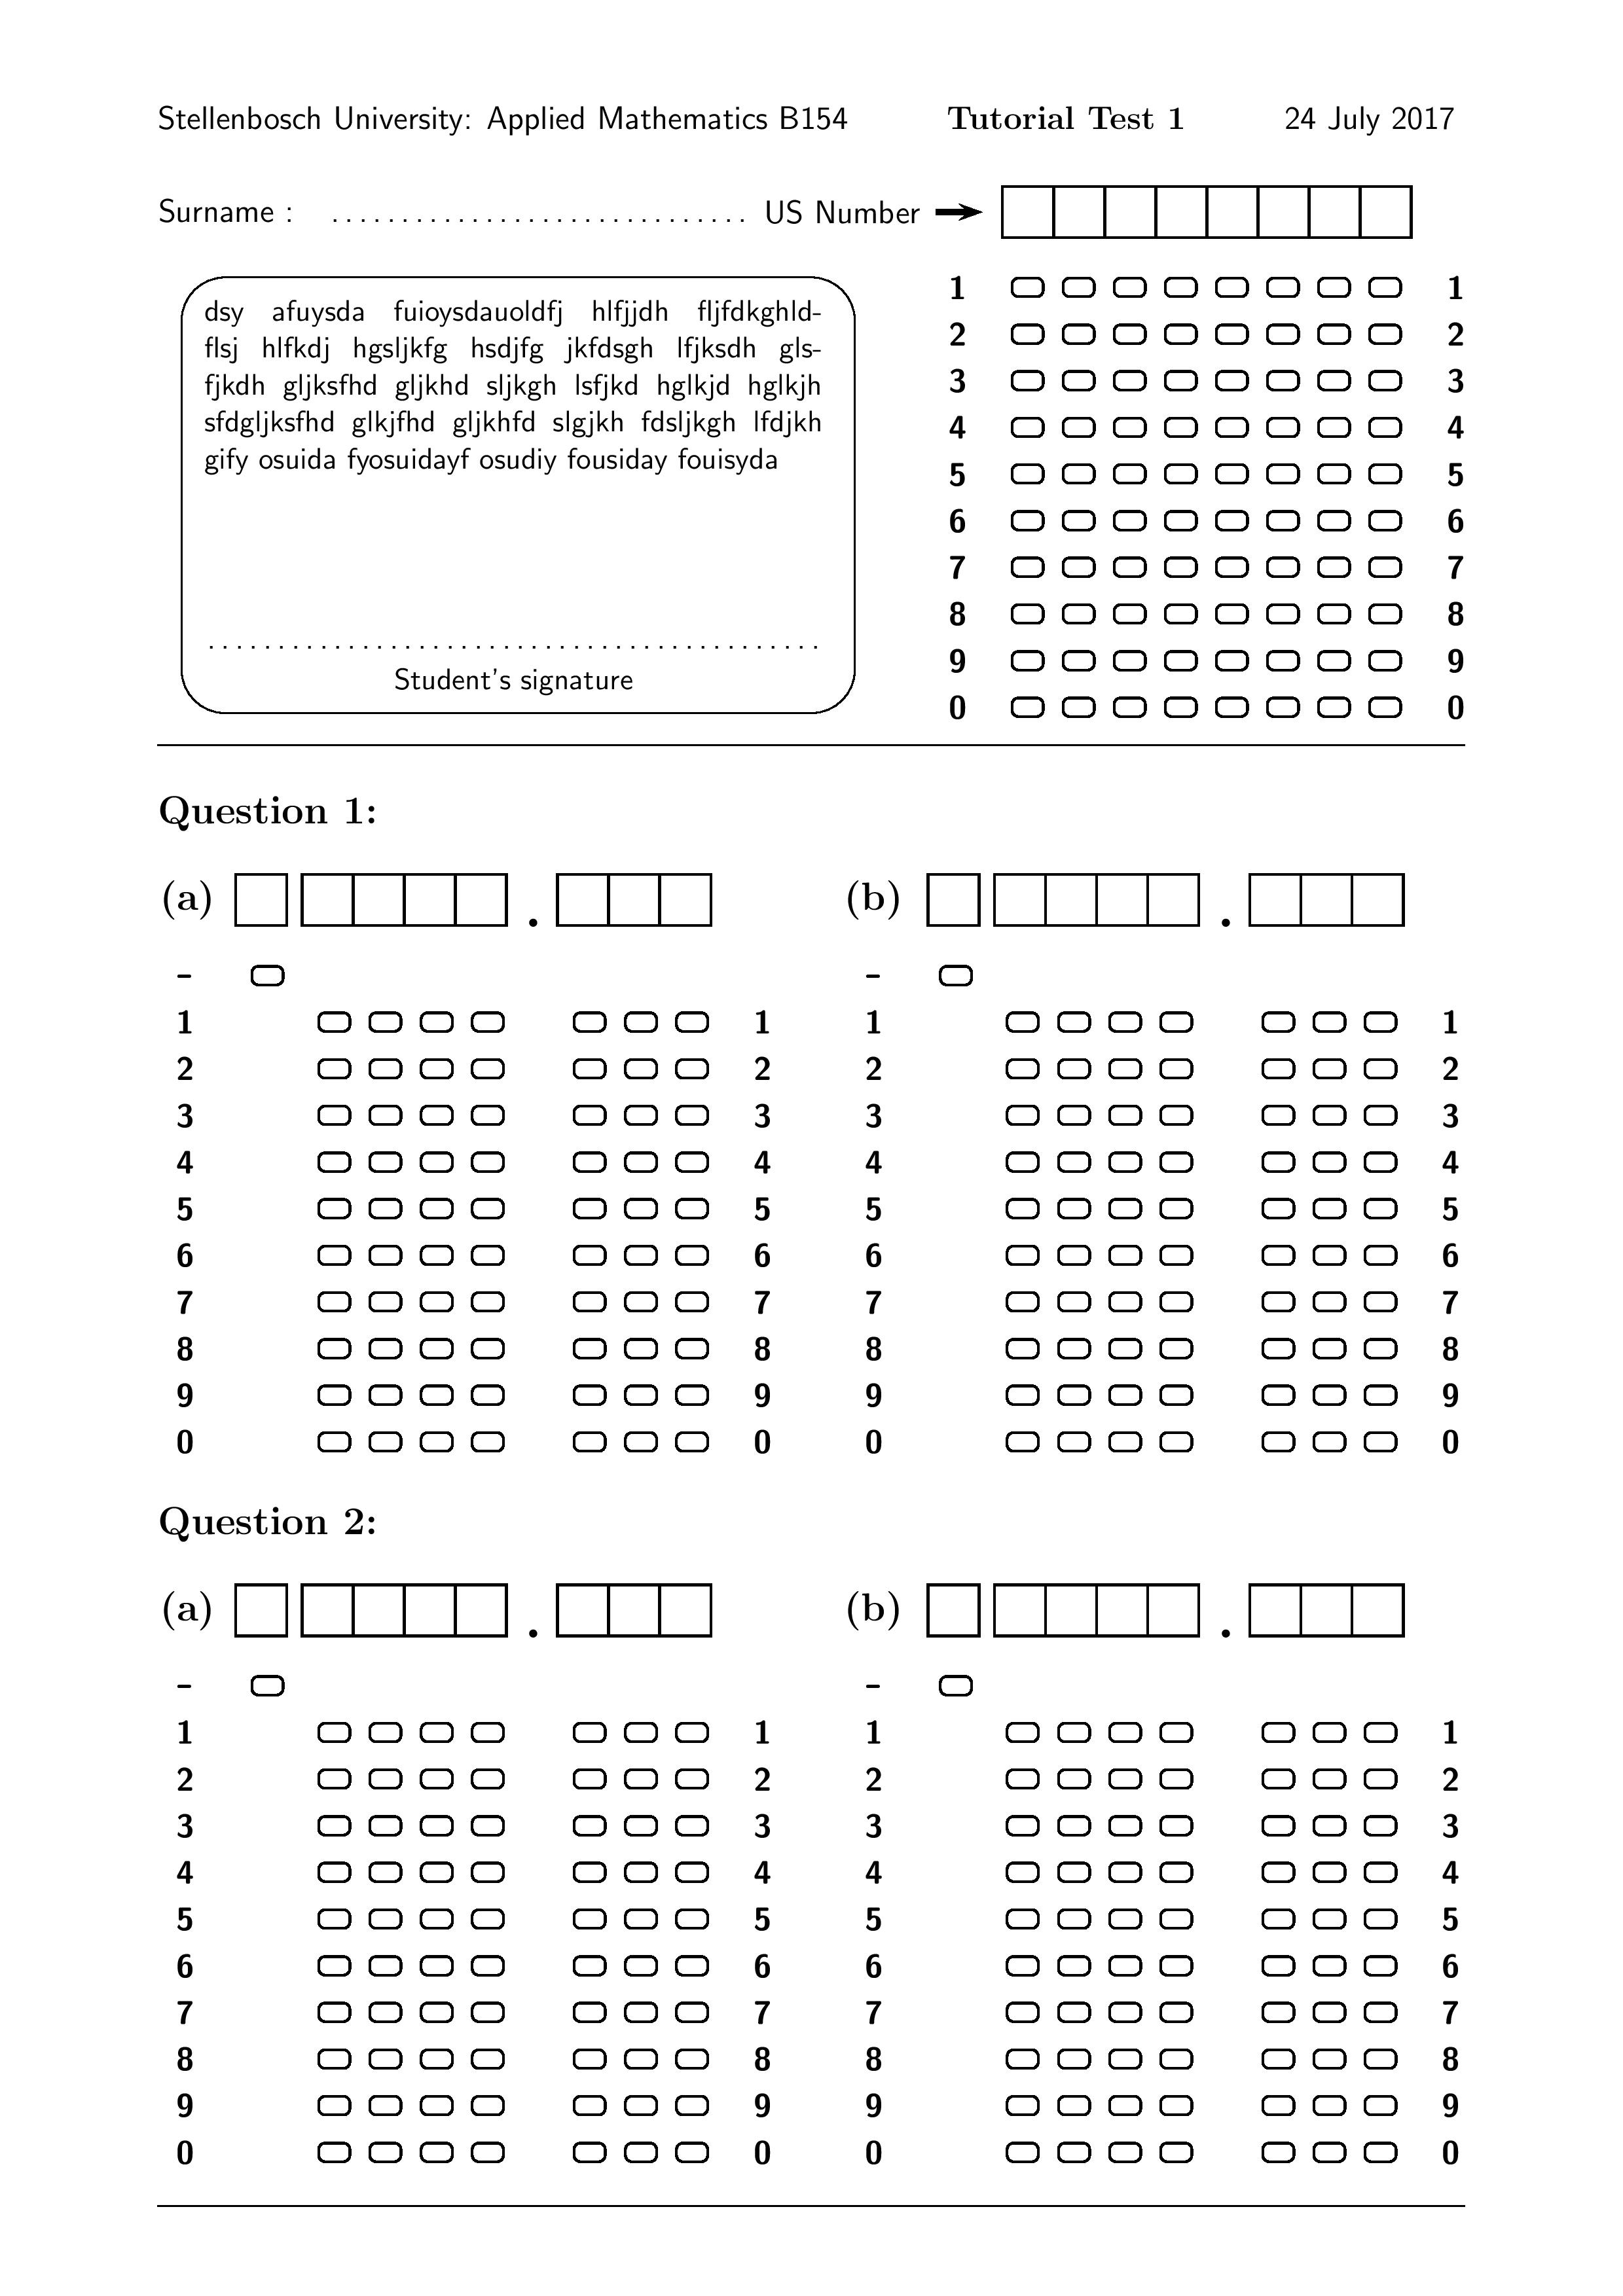
\includegraphics[width=6cm]{NumbersTemplate}\\
  \caption{Automatic test grading template layout.}
  \label{fig:NumbersTemplate}
\end{figure}


Any additional assumptions are specified at the appropriate times throughout this project. In the next section the project objectives is laid out.


\section{Project objectives}
\label{sec:Objectives}

The problem as stated in section \ref{sec:problemStatement}, is addressed by pursuing the following objectives:
\begin{enumerate}
  \item Do a \textsl{literature study} on the topics of \textsl{Image Processing},\textsl{Computer Vision} and \textsl{Character Recognition}. Further a \textsl{literature study} on \textsl{Neural Networks} and \textsl{Probabilistic Graphical models} is also done.
  \item Develop a \textsl{software application} to allow a \textsl{user} to grade a large number (approximately 1000) scanned in student tests automatically.
\item The software should providing precise and useful feedback. To do this every graded result will also include feedback on what questions the student answered incorrectly.
\item Upgrade the software to allow students to cross out answers over having to erase them.
  \item Do a weekly \textsl{validation experiment} with the software, by grading tutorial test for the department. The results are then used as the student's grade for that test.
  \item Use an \textsl{agile development methodology} to improving the software in parallel with the grading of weekly tests.
  \item Add additional software using machine learning to improve the accuracy of the system in grading these test.
  \item Add additional software that allows students to specify their student number only using characters, which makes the template easier to use.
\end{enumerate}

The objectives are covered in different chapters in the report. Note that each objective (1--8) build on the objective(s) previously listed.

 %To increase ease of use, software is developed that provides the option to students to only writing down their student numbers and not use the bubbles. Thus time does not get wasted filling in the student number bubbles. This result is achieved in Chapter \ref{sec:pgmStudentNum}.

\section{Research methodology}

To complete the objectives listed in Section \ref{sec:Objectives}, a agile development methodology is used. The methodology consists of six different phases:
\begin{enumerate}
\item Identify a new feature or update that needs to be implemented into the software package.
\item Do a study on the existing methods to implement this new software.
\item Implement and integrate the new software with the current knowledge of the solution.
\item Test the software and observe if it is working as planned.
\item If the software is not working as planned, revisit steps 2-4 until the new software is working.
\item Use version control, in this case Git, to save the latest version of the software.
\end{enumerate}


Next the structure and graphical overview of the software is presented.

\section{Graphical overview of system}
%\subsection{System overview}

When thinking about the template, from a philosophical sense, it can be represented using 6 information nodes. These nodes are illustrated in Figure \ref{fig:systemOverviewIntro}. The unnamed blocks indicate that information processing happens in these steps. The student has certain information he/she wants to portray on the paper. This includes the 4 answers and student number he/she wants to write down. Thus those 5 nodes gives rise to the image, representing the last node. These nodes have to be represented in a probabilistic way. The reason for this is, because the process of writing answers down and scanning the test sheet in is going to produce a different image every time a test is written, even though the same answers are intended. Thus the system is fundamentally tasked with inferring the probability of each answer and the student's number given that image as evidence. This is done by processing the image evidence to produce and estimate of the intended answers. These processes are described in later sections. In the next section a literature study on current systems is discussed.
\begin{figure}
  \centering
  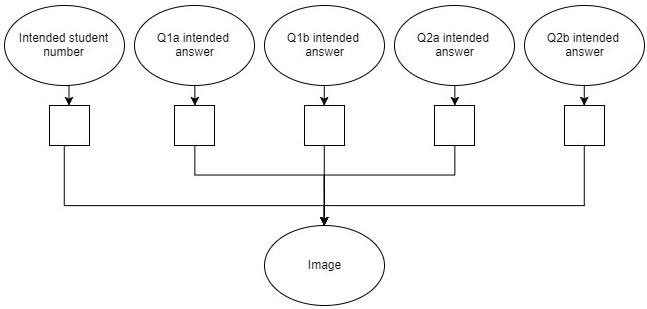
\includegraphics[width=11cm]{systemOverview}\\
  \caption{Graphical overview of the system as a whole.}
  \label{fig:systemOverviewIntro}
\end{figure}

For a more detailed mathematical overview of the system, refer to Appendix \ref{ap:systemOverview}.

%\subsection{Graphical representation}

%For this project a graphical approach is followed in representing the software developed. A graphical model in essence allows software to be represented as information (nodes or circles) and relationships (directed arrows). The directions of the arrows represents what information causes other information to be created, thus given a parent to offspring interpretation). An example of such a graph can again be seen in Figure \ref{fig:systemOverviewIntro}. This allows intuitive reasoning about how the system should operate. An observation is always made in the form of an image and then the system is tasked with predicting what the written answers are. Due to the probabilistic nature of the system a probabilistic component is also needed in this graphical models. Thus a probabilistic graphical model (PGM) is used.

%A PGM is in essence the same as a general graphical model. The only difference is that now the information and relationships between information bubbles are probabilistic and not always certain as with general logic graphical models.

%A literature study is presented next on methods currently used by existing automatic test grading systems. This will describe in the next chapter.        	%Intro
\chapter{Literature study}
\label{ch:LiteratureStudy}
\graphicspath{{Chapter2/Chapter2Figures/}}
In the previous chapter the problem statement and objectives of this project was laid out. Further, a brief system overview was provided.
This chapter will provide information on already existing Optical Mark Recognition (OMR) systems and the techniques they use for conducting image processing. Research on additional machine learning approaches used in character recognition and probabilistic modelling is also given.

\section{Existing Optical Marker Recognition techniques}
An OMR system is software that is used to extracted handwritten information from a filled-in form. Each system normally has a specific template that it can extract information from. An example template is shown in Figure \ref{fig:omrTemplate}. These systems are generally used when fast and accurate grading of tests are required. The black boxes in the figure are used to locate the template. The main drawback of these systems is that information can only be portrayed in a limited manner, due to the bubbles. On an OMR template there is a grid of bubbles that allows a user to choose between different options to answer. OMR systems are thus excellent for the grading of multiple choice type questions. 
\begin{figure}
  \centering
  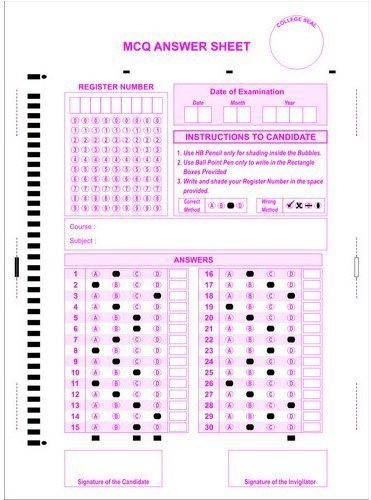
\includegraphics[width=14cm]{omrTemplate}\\
  \caption{Standard OMR template with reference blocks on the left \citep{stdTemplate}.}
  \label{fig:omrTemplate}
\end{figure}

\subsection{Standard Optical Marker Recognition systems}
\label{sec:StandardTech}

As can be seen in Figure \ref{fig:omrTemplate}, there is normally specific reference blocks on an OMR template. These blocks are included to allow the computer vision and image processing algorithms to find the orientation of the image more easily. Other templates include lines that can be used to locate the template.

In an OMR system there are normally two phases in the grading of a test \citep{DraganI2003}. The first step is to determine the grid locations where the answers are located in the image. In this process the system finds the orientation of the template in the image and therefore can approximate the locations of the bubbles. Normally, some preprocessing on a blank template is done beforehand to aid in locating the bubbles. Once the bubbles are found, their estimated locations gets stored. The second step is then to estimate the value of each bubble and use these values as the estimated answers. These steps are described in more detail next.

\subsubsection{Finding the template}

The first process performed by OMR software is to locate a template grid inside the test image. This step is necessary for the software to identify which bubbles corresponds with each answer. One method of locating the template is identifying lines in the template. The border normally contains long lines that can be extracted using a Hough transform \citep{MVGI2015}. A Hough transform is used to locate instances of an imperfect object within a certain shape range. A specific form of a Hough transform can be implemented to detect lines. This form is called a Radon transform \citep{MathWorks}. A Radon transform provides a way of representing an image as a summation of different line integrations.

Once at least two line references on a page have been found, the template orientation can be determined. Those two lines are then used to find two reference points on a page. These points allow the system to estimate the locations of every bubble on the template sheet. In the next section a method to process these bubble is described.

\subsubsection{Processing a bubble}

Once an estimated location for each bubble is known, the next step for an OMR system is to process these bubbles. A basic image processing method to classify bubbles is by adding the number of coloured-in pixels \citep{MVGI2015}. If this value is above a specific threshold value, the bubble is classified as filled-in, otherwise not. An additional algorithm is needed to detect if a bubble is crossed out .

In this project additional contour detection is used to determine if an answer in a bubble is truly coloured in and not just crossed out. This means that the contour around the bubble needs to be detected and used in the analysis. In Python (or C++) this can be implemented using the freely available OpenCV library \citep{AdrianR2016}. OpenCV is an image processing library that has highly optimized techniques to find contours in a given image. An example of this is shown in Figure \ref{fig:Cross}. Once the contour information is known, the bubbles can be assessed by the pixels inside it, as well as its shape. Thus by evaluating the shape of a contour it can be determined if a bubble is crossed out or not.
\begin{figure}
  \centering
  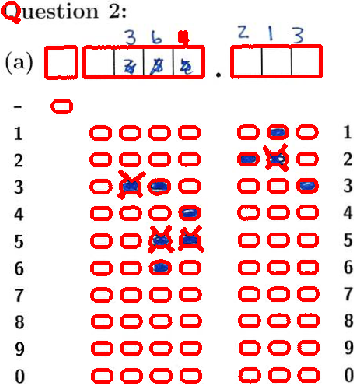
\includegraphics[width=5cm]{Cross}\\
  \caption{Contours found around corrected answer.}
  \label{fig:Cross}
\end{figure}

\section{Optical character recognition}
\nomenclature[A]{$OCR$}{Optical character recognition}
\nomenclature[A]{$DCNN$}{Deep convolutional neural network}
\nomenclature[A]{$MNIST$}{Modified national institute of standards and technology}
Optical Character Recognition (OCR) software is also needed and applied on the characters blocks present on the templates, to further increase the accuracy of the system. It is found that one preferred way of performing OCR is using TensorFlow. This method is described by \citet{Tensor}. TensorFlow is a Python library, but allows the building of instructions to be implemented in ef{f}icient C++ code. For this test grader, TensorFlow is used to construct a deep convolutional neural network (DCNN). Deep convolutional neural networks are powerful machine learning techniques generally used to process images. One effective application of a DCNN is that it is excellent at processing an image containing a digit and estimating that digit.

\subsection{Probabilistic approach}
A last piece of information that needs to be investigate is how the bubble and character evidence can be brought together in an effective way to produce the best estimate of the intended student entries. Once a bubble and character are analysed, a probabilistic value is assigned to it. Each bubble has a probability of being filled in, while each character has a probability distribution over 10 digits. A probabilistic model is needed to predict these student entries. In \citet{pgmPy}, a machine learning approach is used to infer a probability of random variables being in a certain state given evidence. This method is known as a Probabilistic Graphical Model (PGM). A \textsl{Probabilistic Graphical Model} (PGM) is a probabilistic framework that consists of a graph that specifies the probabilistic relationship between a number of random variables. These types of models work well in some aspects of the medical field. If a patient has certain symptoms, a PGM can be used to predict what the underlying illness behind the decease is. In this project a PGM is used to estimate the underlying student entries given the evidence presented. The library used by \citet{pgmPy} is called pgmpy. This library allows for a PGM to be constructed in Python. 

\section{Conclusion: System requirements}
In conclusion it is seen that a combination of image processing and machine learning techniques is needed to successfully grade a student test paper. A good method in locating a template is using a Radon transform to find reference lines on an image. Once this is done, the bubbles can be estimated in the image. It is found that a DCNN can be implemented to classify digits in the TensorFlow library environment. Once all these evidence are acquired, a PGM was found to be a preferred method in predicting the estimated entry answer of the student.
In the following chapter, a more detailed overview on the image processing techniques used in this project is given.
			%Literature study
\chapter{Image Processing}
\label{ch:ImageProcessing}
\graphicspath{{Chapter3/Chapter3Figures/}}
The previous chapter focused on existing methods of grading tests automatically. It was found that most systems only use image processing, without a machine learning component, to grade these test. In this chapter the core techniques behind processing these answer sheets, using image processing, is described. By using only these image processing techniques a reasonably accurate system can already be constructed.

For further improvements in accuracy we and implement two machine learning approaches. These approaches are discussed in Chapter \textbf{\ref{ch:MachineLearning}}.

\section{Orientation Detection}
\label{sec:orientDetect}
As mentioned in Section \ref{sec:StandardTech}, there are two main steps in OMR grading. The first challenge with grading a scanned in answer sheet, is finding the orientation of the template in the image. To do this 2 or more references points must be found on the page. These reference points then allows for the calculation of the template's rotation, offset and size inside the image. In Chapter \ref{ch:LiteratureStudy} it was found that the traditional way to find this reference points was to include them on the page, in forms of black blocks or lines. Including black blocks is an effective method of finding the template, but might look a bit less attractive, due to the black blocks on the page.

For this project the markers or reference points that the software uses are already present on the template paper. These are the two longest horizontal lines as well as the two vertical lines on the comment box, as can be seen in Figure \ref{fig:radonResults}. Together these lines have enough information to determine 4 reference points, shown in red in the figure. The reason these lines are chosen as references, are due to the fact that a Radon transform can easily be applied to find them, as seen in Section \ref{sec:RadonTransform}. Thus the software can successfully find the template even though one of the 4 lines are identified incorrectly. Using the reference points the rotation, offset and size of the template is calculated. But before the orientation of the image can be determined it is a good idea to quickly check if the image might be upside down. This is done to make it easier to find the orientation afterwards. To do this some initial image filtering is firstly required and is discussed in the next section.

\begin{figure}
  \centering
  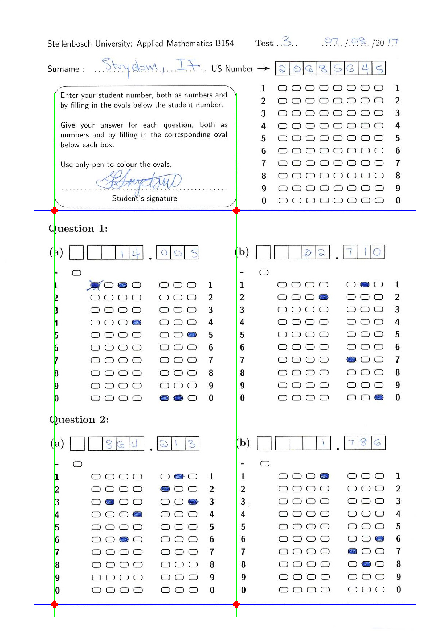
\includegraphics[width=7cm]{RadonResults}\\
  \caption{Four markers found from applying Radon transforms.}
  \label{fig:radonResults}
\end{figure}

\subsection{Initial filtering and orientation detection}
\label{sec:InitImageFilter}

To check if and image is upside down the software first needs to find relevant contours on the page. The contours are then filtered out if it does not loosely match the characteristics of a bubble or character block. This process can be described in 5 steps:

\begin{enumerate}
\item Threshold the image by making all the pixel values either white (lower that the mean) or black (higher that the mean).
\item Do contour analysis on the image to find all the contours, using the python library OpenCV.
\item Filter through the contour array to filter out all contours that are not approximately the size and aspect ratios desired.
\item Save these contours for later use.
\item Determine if more contours lie above the middle of the image. This is true if the image is the right way around. Rotate the image by 180$^{\circ}$ otherwise.
\end{enumerate}

It is important to note that there are still unwanted contours in the list, but for now this reduced list is sufficient. Once the list is found the software counts the number of contour centrepoints below and above the image center. Figure \ref{fig:reduced} shows the resulting contours found in the image. As can be seen in the figure more bubbles should be below the horizontal center line, for the image to be the right side up. The next step will now be to determine the coordinates of the answers the student wrote down. To do this the template is first located in the image. This process is described in Section \ref{sec:RadonTransform}.

\begin{figure}
  \centering
  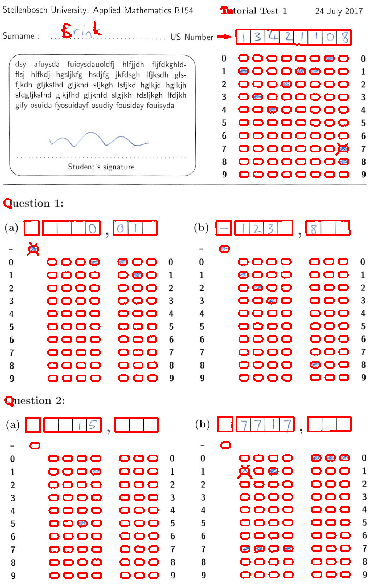
\includegraphics[width=7cm]{Reduced}\\
  \caption{Reduced contours in image.}
  \label{fig:reduced}
\end{figure}

\subsection{Radon Transform}
\label{sec:RadonTransform}
\nomenclature[S]{$G(r,\theta)$}{Radon transform defined over $r$ and $\theta$}
\nomenclature[S]{$f(x, y)$}{Two dimensional function that a Radon transform is applied over}
The Radon transform is an integral transform that can be represented by a series of line integrals over a function $f(x,y)$. These transforms are commonly used in CT scans. Mathematically this transform is defined as $$G(r,\theta) = \int_{-\infty}^{\infty} \int_{-\infty}^{\infty} f(x, y) \delta(x\cos(\theta) + y\sin(\theta) - r) dx dy.$$Where $r$ represents the perpendicular offset of the line and $\theta$ the angle of the line. $x$ and $y$ represents variables within a 2 mentionable space within which the function $f(x,y)$ is defined.  A visual interpretation of this transform can be seen in Figure \ref{fig:RadonT}.  

\begin{figure}
  \centering
  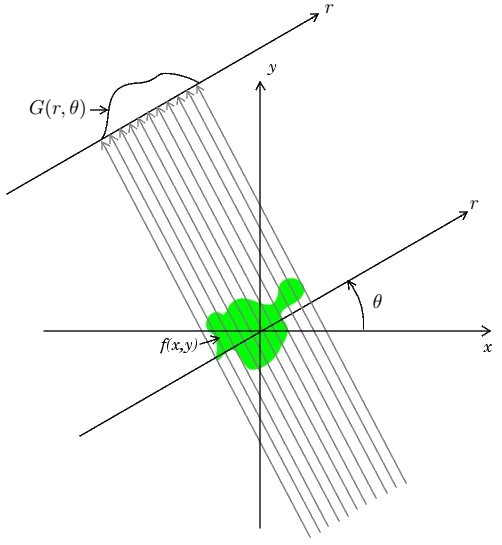
\includegraphics[width=8cm]{RadonT}\\
  \caption{Radon transform applied on a 2 dimensional space, from \citet{radon}}
  \label{fig:RadonT}
\end{figure}

\subsection{Finding the template}
\label{sec:findTemplate}

In this project the image's Radon transform is calculated for specific intervals of the gradient. Each gradient interval will thus generate a 1 dimensional array of values corresponding with the pixel intensities along the lines that are being summed, as seen in Figure \ref{fig:RadonT}. This method is used determine where the 2 horizontal and 2 vertical lines are located, as mentioned in Section \ref{sec:orientDetect}. 

To find the first two horizontal lines the Radon transform's values are calculated between the angles 85$^{\circ}$ and 95$^{\circ}$. It is amused that the image will not be rotated by more that 5$^{\circ}$ in either direction. Black lines will cause a spike to appear on the Radon transform for the angle where it is summing parallel with that black line. Thus by finding the transform angle value that present this maximum value, the rotation of the template can be found. The two maximum values that is recorded at this angle is then recorded as the relative locations of the two horizontal lines. After the correct angle is found the two vertical lines can be found by applying a Radon transform at a angle 90$^{\circ}$ clockwise from the previously calculated angle. The two peak values at that angle then provides the relative locations of the two vertical lines.The four reference points can now be calculated, as seen in Figure \ref{fig:radonResults} can be calculated. Once the reference points are found the image is rescaled and orientated to the original template size for further processing. In Figure \ref{fig:rotate} the corrected image is shown.

\begin{figure}
  \centering
  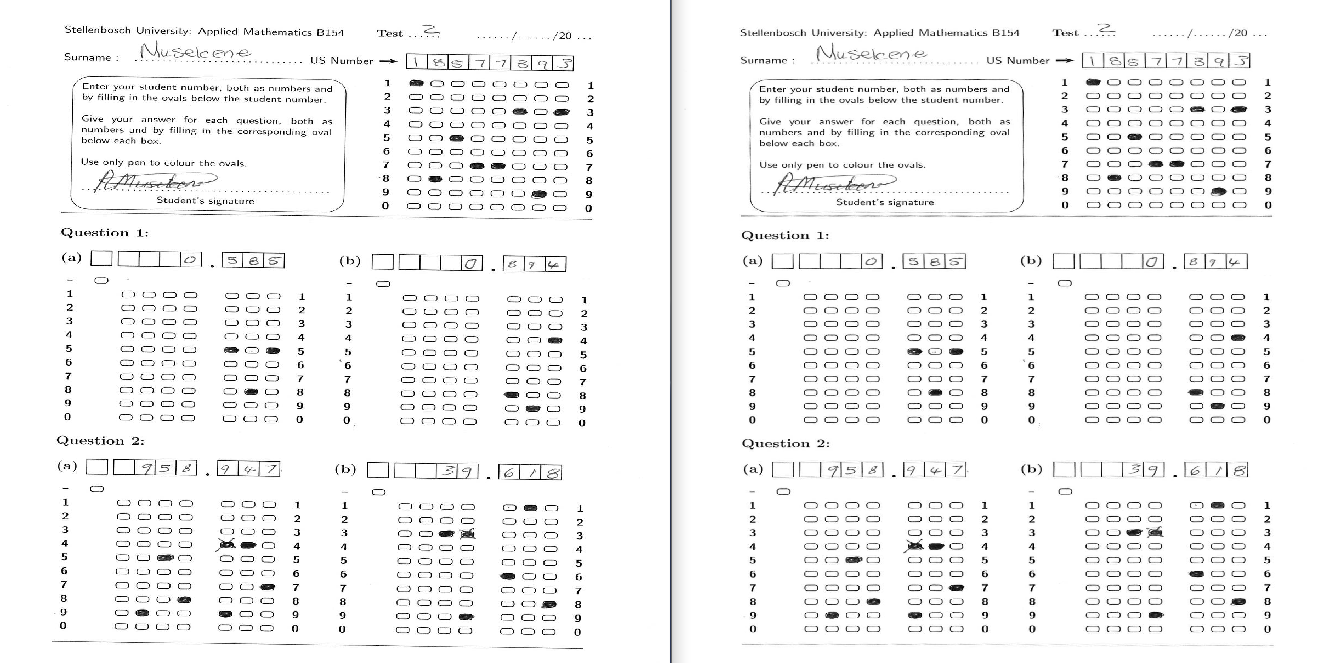
\includegraphics[width=14cm]{Rotation}\\
  \caption{Result in rotation after applying radon transform.}
  \label{fig:rotate}
\end{figure}

Once the template is found the bubble values and digit blocks can be determined, using reference location. These reference locations were calculated in preprocessing done on an empty template. Figure \ref{fig:FinalEstimate} illustrates the final estimation of all the bubbles in the template. The estimated bubble centres are coloured red, while the green points represent the centres of all the remaining contours.

\begin{figure}
  \centering
  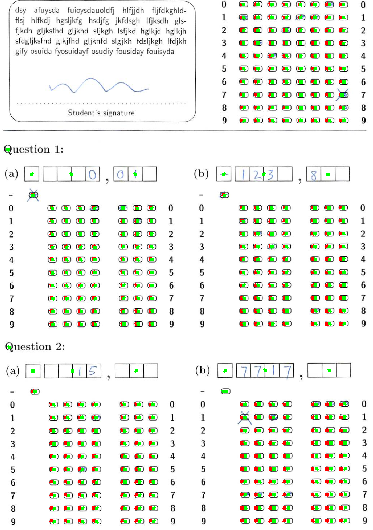
\includegraphics[width=6cm]{FinalEstimate}\\
  \caption{Detection of contours in image and estimation of bubble locations.}
  \label{fig:FinalEstimate}
\end{figure}

Now that a list of possible bubble contours are found with the estimate bubble centres, one contour needs to be assigned to each bubble. This is discussed in the next section.

\section{Bubble detection and processing}
\nomenclature[S]{$n$}{Number of bubbles of template sheet}
To find the location of each bubble in the image, the system simply takes the contour closest to the estimated bubble location. This can be done in an efficient manner by sorting the contours by their locations. Searching through the contours now becomes linear and of complexity $O(n)$, where n is the number of bubbles. This means that the processing time to find these bubbles is linearly related to the number of bubbles in the template image. 

Next the data in each contour needs to be processed and stored. The first type of evidence is calculating the average pixel intensity inside the contours. If this value is high the bubble is most likely coloured in or crossed out. The advantage of using the closest contour as the bubble's estimated location, over conventional methods now becomes apparent. In conventional methods an estimated area is calculated where the bubble is most likely to be located. This becomes problematic if the system needs to know if the bubble has been crossed out, as only data about pixel intensities are present. 

Using contour analysis, information about the shape of the bubble entry is also provided. Thus by drawing the smallest possible block around the contour, that still covers every value inside the contour, an area can be calculated. This area becomes large when a answer is crossed out, due to the lines stretching outside the initial bubble. By inspecting the area value, the system can successfully determine if the bubble is filled in and crossed out.

\section{Data processing and grading}

The previous section now allows each bubble to be classified into 3 categories namely, empty, completely filled in and crossed out. An additional category of partially filled in will also be introduced, as it aids grading of tests where students write lightly. An algorithm to determine what bubble was chosen can now be described as follows:

\begin{enumerate}
\item Start with column 0.
\item Count the number of completely filled in answers in this column. Store the position of that entry for later use.
\item If there are no completely filled in answers, count the amount of partially filled in answers and override the previous values.
\item If the previous result is 0, set the output value for that column to 0.
\item If step 2 or 3 presents a value greater that 1, save the answer sheet to a clash list to be evaluated manually once the automatic grading of the test are completed.
\item Repeat steps 2 to 5 for each column in the bubble grid.
\end{enumerate}

This algorithm thus checks if there are more that one entry in any of the columns. If this is true the results is sent to a clash list to be marked manually. If one one bubble was found to be coloured in the value gets set to the index of that bubble. Finally if no bubbles where coloured in the result for that column gets set to 0.

\section{Conclusion}

This chapter provided an overview of a basic automatic test grading system using image processing and computer vision. The system can achieve acceptable results using only these techniques.

The following chapter will focus on applying additional machine learning techniques to further improve the accuracy of grading these test.			%Image processing
\include{Chapter4/chapter4}			%Machine learning approach
\include{Chapter5/chapter5}			%Results
%\include{Chapter6/chapter6}
%\include{Chapter7/chapter7}

\def\baselinestretch{1}
\chapter{Summary and conclusions}
\label{ch:Conclusions}

\graphicspath{{Conclusions/Figures_Conclusions/}}
\section{Project summary}
In this project an automatic test grading system was developed with the aim of grading student test using a special template. Initially, research was done into excising methods of grading these tests automatically. It was found that normally only image processing methods are used to grade bubbles on a paper. For this project additional machine learning capabilities were built into the system. This allows for a better estimation of what the student  intended to write down on the paper.

\section{How this final year project benefits society}
In the African society there is a great number of individuals who do not have access to quality educational opportunities. The educational systems these individuals do have are normally not up to standard with limited teaching assistance. Educators who are available are not always accessible to learners to provide quality education. Automatic Mark Recognition software like the one developed in this project allows for a large number of tests to be assessed automatically and accurately in a short time span. This assists educators in handling bigger classes and thus provide more learners the opportunity for a better education.

\section{What the student learned}
During the execution of this project, the student learned that time management is important to complete a project of this scale. Time management also allows an individual to continuously asses how he/she is doing with respect to a schedule. This not only increases performance, but also self confidence in the final product. Finally, the student learned how to develop a software package in a professional environment. This project also allowed the student to gain a basic knowledge on a broad range of fields including image processing, neural networks and probabilistic graphical models. 


\section{Future improvements}
To increase the speed of grading tests it should be considered to use Stellenbosch's custom PGM library, implemented in C++. By continuously updating the estimated orientation of the template as more bubble contours gets classified, accuracy in finding these bubbles can be increased. Further increases in test grading speed can be achieved by only doing image processing on the expected locations of the bubbles. This will bring some extra technical hurdles, but can increase the software's speed. Further the accuracy of the character recognition neural network can be increased by making use of Generative Adversarial Networks (GAN) to train the network on actually classified test results.

\section{Summary and conclusions}
For 890 tests the system takes approximately 30 minutes to grade these tests. This time is acceptable for the department, because it allows for more flexible answers. For example, a student number can be identified by only referring to the characters written in the student number box. The system has an overall accuracy of 97.1\% with only automatic grading. An additional feature is implemented that transfers tests which the system is uncertain about, to a user to manually grade. Combined with the human operator, only 1 test in every tutorial session (average of 890 tests) gets graded incorrectly. In combination with the manually checked tests, the system thus obtains a 99.9\% accuracy on grading tests correctly, while still allowing students greater flexible in the methods of answering these tests.	%Conclusion

%\bibliographystyle{natbib}
\renewcommand{\bibname}{References} % changes default name Bibliography to References
%NB! Hierdie path moet reg wees op jou laptop! Die dotjies (..) is om 'n relatiewe pad laer in die
%hierargie aan te dui. Gebruik forward slashes en nie backslashes nie!
\bibliography{C:/Users/User/Desktop/MyFolders/Universiteit/Skripsie/FinalReport/LatexReport/V7MachineLearning/References/references}
%Jy kan ook die references aandui met 'n volledige path:
%\bibliography{C:/Users/User/Desktop/MyFolders/Universiteit/Skripsie/FinalReport/LatexReport/V2/References/references}

% I took this style form the Journal of Microbiology, you may use your own. See the user manual of
% the natbib style by Patrick Daly.
\bibliographystyle{Classes/jmb}
\addcontentsline{toc}{chapter}{References} %adds References to contents page

\appendix
\chapter{Overview of system}
\label{ap:systemOverview}
\graphicspath{{Chapter1/Chapter1Figures/},{Chapter4/Chapter4Figures/}}

In this chapter a graphical and mathematical derivation of the entire system is given.

\section{System as a whole}

\begin{figure}
  \centering
  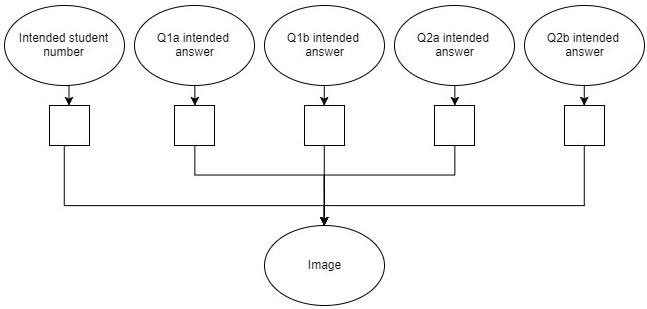
\includegraphics[width=11cm]{systemOverview}\\
  \caption{System overview.}
  \label{fig:systemOverview}
\end{figure}

As described in Chapter \ref{ch:Introduction}, the system can fundamentally be represented with 6 information nodes. These nodes are shown in Figure \ref{fig:systemOverview}. The student has certain information he/she wants to portray on the paper. This includes the 4 answers and student number the student wants to write down. Thus those 5 nodes gives rise to the image, representing the last node. Thus fundamentally the system is tasked with working out these 5 conditional probabilities: $P(StudentNumber/Image)$, $P(Answer1/Image)$, $P(Answer2/Image)$, $P(Answer3/Image)$ and $P(Answer4/Image)$. The random variables StudentNumber and Answer(1 to 3) thus represent all the possible values that the student number and answers possibly can be. The image is a random variable representing the total number of possible states the image can represent. This value is in the order of 1240*1754*256 possible states. To practically represent this further assumptions are made in the following sections. 
 
The aim of the software is to maximize the likelihood of those probability distributions indicating the correct answers.
The reason the problem is represented in a probabilistic way is due to the fact that different images are going to be generated every time a test is written. This is true even when the same information is going to be portrayed. Everytime a student writes a test he/she is going to write in different ways. A probabilistic graphical model (PGM) is thus used to describe this system and its inner operations. For a more detailed explanation on PGM's, refer to Section \ref{sec:PGM}.  The blocks in Figure \ref{fig:systemOverview} represent additional processing that is described in the following sections.

To calculate those 5 probabilities, some more detailed derivations are necessary. These derivations are described in the next section.

\section{Deriving the intended student entry}

\subsection{Student answer}

In Section \ref{sec:pgmStudentNum} it was determined that the student answer can be calculated by combining the intended sign and digits of each column to form an answer. The reason for this could be attributed to the fact that these digits where independent of one another. This means that the intended digit in a certain column is not influenced by what the values in other columns are. In Equation \ref{eqn:ansIndep} this independence property can now be seen. To find the most probable answer only $P(sign/Image)$ and $P(digit(1-7)/Image)$ still needs to be calculated. Using the image processing techniques described in Section \ref{ch:ImageProcessing} the $P(sign/Image)$ can simply be determined heuristically by determining the probability of the bubble being coloured in, underneath the sign. Thus the only values yet to calculate is $P(digit/Image)$. This is described in Section \ref{sec:digit}.

\begin{align}
% \nonumber to remove numbering (before each equation)
  P(Answer/Image) =  P(sign/Image)*P(digit1/Image)*...*P(digit7/Image)
\label{eqn:ansIndep}
\end{align}

\begin{figure}
  \centering
  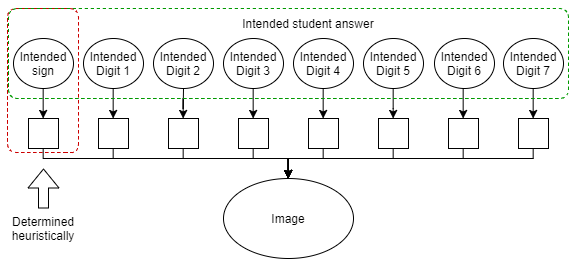
\includegraphics[width=10cm]{ans}\\
  \caption{Graphical setup of determining student answer.}
  \label{fig:ans}
\end{figure}

\subsection{Student number}

As state in Section \ref{sec:pgmStudentNum} the assumption of independence does not hold in the case of a student number. The reason for this is, because every 8 digit number is not equally likely to be a student number. Only student numbers that are valid will be considered as a possible state that the student number node can take on. This node will have $+- 900$ states, depending on the number of student numbers. The student number graph can be seen in Figure \ref{fig:stdNum}. Next a derivation for $P(studentNumber/Image)$ is needed. 

In the below equations, 'Digits' represents the 8 digit random variables. The first step is to apply Bayes rule as seen in Equation \ref{eqn:bayesStd}.

\begin{align}
  P(StudentNumber,Digits/Image) =  \frac{P(Image/StudentNumber,Digits)*P(StudentNumber,Digits)}{P(Image)}
\label{eqn:bayesStd}
\end{align}

When all the digits are known, the image becomes independent of the student number. This can be seen in Equation \ref{eqn:bayesStd}. Also the chain rule states that Equation \ref{eqn:chain} must be true.

\begin{align}
  P(Image/StudentNumber,Digits) = P(Image/Digits)
\label{eqn:digitInd}
\end{align}

\begin{align}
  P(StudentNumber,Digit) = P(Digit/StudentNumber)*P(StudentNumber)
\label{eqn:chain}
\end{align}

Next the Digit random variable is summed out to produce $P(studentNumber/Image)$, as seen in Equation \ref{eqn:sumRule}.

\begin{align}
  P(StudentNumber/Image) = \sum_{D}^{All} \frac{P(Image/Digits)*P(Digit/StudentNumber)
  *P(StudentNumber)}{P(Image)}
\label{eqn:sumRule}
\end{align}

Applying Bayes rule again the following equality can be presented, as seen in Equation \ref{eqn:bayesStd2}.

\begin{align}
  P(StudentNumber/Image) = P(Image/Digits) = \frac{P(Digits/Image)*P(Image)}{P(Digits)}
\label{eqn:bayesStd2}
\end{align}

Thus the result can be seen in Equation \ref{eqn:final}. $P(StudentNumber)$ can be taken out of the sum, due to it being independant of $Digits$.

\begin{align}
  P(StudentNumber/Image) = P(StudentNumber)*\sum_{D}^{All} \frac{P(Digits/Image)
  *P(Digits/StudentNumber)}{P(Digits)}
\label{eqn:final}
\end{align}

$P(StudentNumber)$ can be initialized as a equal distribution, because every student number is equal as likely to be in a given test. $P(Digits/StudentNumber)$ is a value that is trained from data. This value symbolizes the probability that the user intended to write down a given digit given that student's student number. This number is thus strongly correlated with the student number. If the first digit of the student number is 1, Digit1 will have a high probability of being 1. The only values that still needs to be calculated are thus $P(Digits/Image) = P(Digit1/Image)*...*$. This derivation is covered in the next section.

\begin{figure}
  \centering
  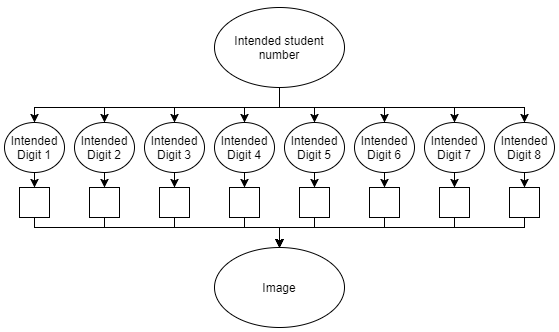
\includegraphics[width=10cm]{stdNum}\\
  \caption{Graphical setup of determining student number.}
  \label{fig:stdNum}
\end{figure}

\section{Deriving the estimated digit}
\label{sec:digit}



\begin{figure}
  \centering
  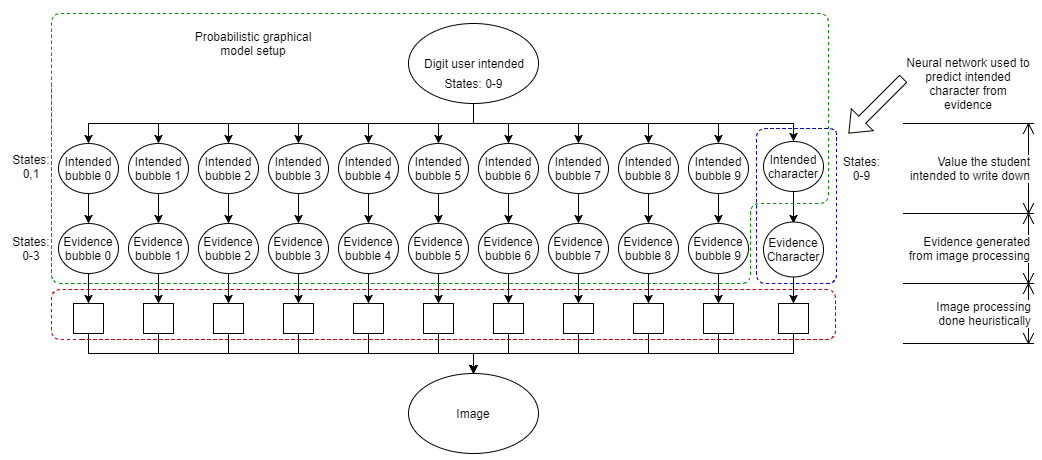
\includegraphics[width=16cm]{pgmDigit}\\
  \caption{Graphical setup of determining intended digit.}
  \label{fig:pgmDigit2}
\end{figure}
 %Graphical overview of system
\chapter{Outcome compliance}
\label{ap:outCompliance}
\graphicspath{{Appendix2/Appendix2figures/}}

Maak die kulomme oucomes, chapters, description

\begin{tabular}{|p{8.3cm}|p{2.7cm}|p{1.5cm}|}
\hline
\textbf{Outcome}&\multicolumn{2}{|l|}{\textbf{Reference}}\\
\hline
& Sections & Pages\\
\hline
1. Problem solving: Demonstrate competence to identify, assess, formulate and solve convergent and divergent engineering problems creatively and innovatively. & \textit{All} & \textit{All}\\
\hline
5. Engineering methods, skills and tools, including information technology: Demonstrate competence to use appropriate engineering methods, skills and tools, including those based on information technology. & \textit{2, 3, 4, 5, 6 \& 7} & \textit{10 -- 62}\\
\hline
6. Professional and technical communication: Demonstrate competence to communicate ef{f}ectively, both orally and in writing, with engineering audiences and the community at large. & \textit{All} & \textit{All}\\
\hline
9. Independent learning ability: Demonstrate competence to engage in independent learning through well developed learning skills. & \textit{2, 3, 4 \& 5} &  \textit{10 -- 37}     \\
\hline
10. Engineering professionalism: Demonstrate critical awareness of the need to act professionally and ethically and to exercise judgment and take responsibility within own limits of competence. &\textit{8.3 \& 8.4}  &  \textit{66 -- 67}        \\
\hline
\end{tabular}

% ------------------------------------------------------------------------

%%% Local Variables:
%%% mode: latex
%%% TeX-master: "../thesis"
%%% End:
 %Mathematical derivation of whole system
\chapter{Mathematical and graphical description of system}
\label{ap:systemOverview}
\graphicspath{{Appendix3/Appendix3Figures/},{Chapter1/Chapter1Figures/},{Chapter4/Chapter4Figures/}}

In this appendix a graphical and mathematical derivation for the system is given. It is shown through mathematical derivation how the pgmpy software can predict the student number and answer given the probability distributions and evidence. It should be noted that the software exploits additional methods in calculating these values in an efficient manner.

\section{High-level overview}

\begin{figure}
  \centering
  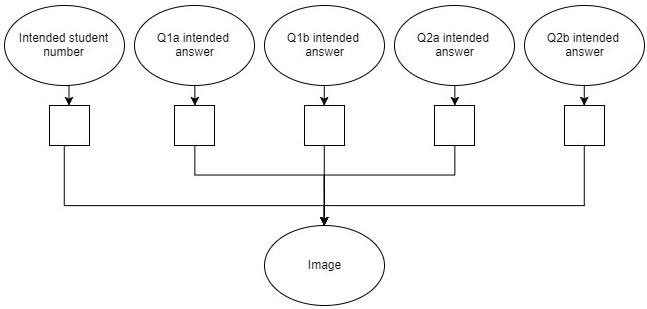
\includegraphics[width=11cm]{systemOverview}\\
  \caption{System overview.}
  \label{fig:appOverview}
\end{figure}
\nomenclature[S]{$A$}{Random variable representing an answer for a specific question}
\nomenclature[S]{$I$}{Random variable representing the test image}
\nomenclature[S]{$S$}{Random variable representing the possible student number}
As described in Chapter \ref{ch:Introduction}, the system can fundamentally be represented with 6 information nodes. These nodes are shown in Figure \ref{fig:appOverview}. The student has 5 pieces of information that he/she wants to portray, signifying the first 5 nodes. Those 5 nodes give rise to the image, representing the last node. At its core the system is tasked with inferring two types of conditional probabilities namely $P(S/I)$ and $P(A/I)$. The random variables $S$ and $A$ represent all the possible values that the student number and answers can possibly have. The image, $I$, is also a random variable representing the total number of possible states the image can take. Each image has a width and length of 1 240 by 1 754 pixels. For every pixel there are 256 possible values, ranging from 0.0 to 1.0. Thus the number of possible images are in the range of 1 240 $\times$ 1 754 $\times$ 256. To practically represent this, more detailed derivations and assumptions is needed. These derivations are described in the next sections. 
 
%The aim of the software is to maximize the likelihood of those probability distributions indicating the correct answers.
%The reason the problem is represented in a probabilistic way is due to the fact that different images are going to be generated every time a test is written. This is true even when the same information is going to be portrayed. Everytime a student writes a test he/she is going to write in different ways. A probabilistic graphical model (PGM) is thus used to describe this system and its inner operations. For a more detailed explanation on PGM's, refer to Section \ref{sec:PGM}.  The blocks in Figure \ref{fig:systemOverview} represent additional processing that is described in the following sections.

\section{The student answer}
In Section \ref{sec:studentAnswer}, it was determined that the student's answer can be calculated by combining the intended sign and digits of each column separately. This is attributed to the fact that these digits are independent of one another, as seen in Figure \ref{fig:appAns}. 

\begin{figure}
  \centering
  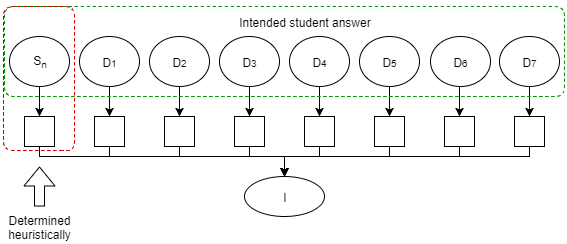
\includegraphics[width=10cm]{appAns}\\
  \caption{Graphical setup of determining student answer.}
  \label{fig:appAns}
\end{figure}
\nomenclature[S]{$Sn$}{Random variable representing the sign of a specific answer}
\nomenclature[S]{$D_i$}{Random variable representing a digit in column $i$ for a answer or student number block}
The intended digit in a certain column is not influenced by what the values in the other columns are. This independence property is thus described by\begin{align}
% \nonumber to remove numbering (before each equation)
  P(A/I) =  P(Si/I)P(D_1/I)...P(D_7/I),
\label{eqn:ansIndep}
\end{align}
where $A$ and $I$ again represent an answer  for a specific question and the image, respectively. The random variable $Si$ represents the sign of the answer.

To find the most probable answer, only $P(Sn/I)$ and $P(D_{1-7}/I)$ need to be calculated. Using image processing techniques described in Section \ref{ch:ImageProcessing}, $P(Si/I)$ can simply be determined heuristically by determining the probability of the bubble being coloured in, underneath the sign. Thus the only values yet to calculate is $P(D_{1-7}/I)$ and derived in the next section.

\section{The intended digit}

\begin{figure}
  \centering
  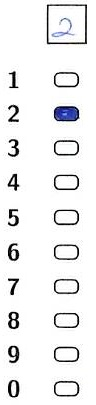
\includegraphics[width=1cm]{column}\\
  \caption{Column with evidence that gets considered for the calculation of an intended digit.}
  \label{fig:column}
\end{figure}

In determining an intended digit there are 11 information nodes to use as evidence. These nodes represent the 10 bubbles and character block, as shown in Figure \ref{fig:column}. Extra nodes are also added to symbolise the intended bubbles as described in Section \ref{sec:studentDigit}. The first bubble might sometimes incorrectly be associated with digit 0. Thus even if the student intended the digit 0 as an answer, the intended bubble of that student was actually the bubble for digit 1.

\begin{figure}
  \centering
  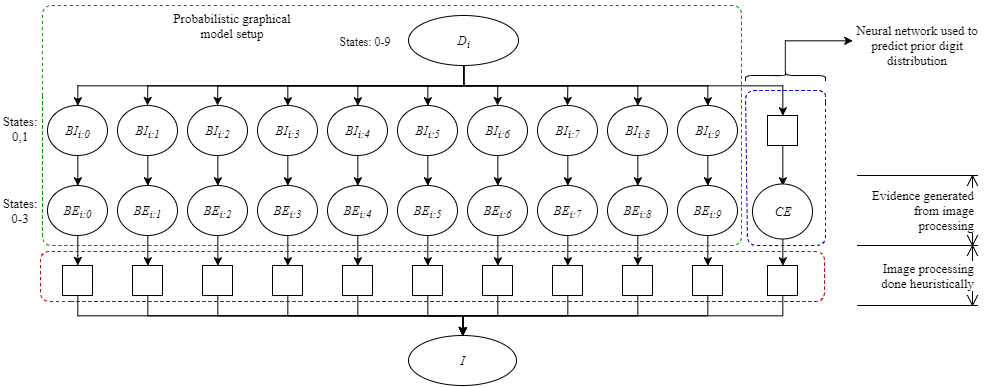
\includegraphics[width=16cm]{appDigit}\\
  \caption{Graphical setup of determining intended digit.}
  \label{fig:appDigit}
\end{figure}
\nomenclature[S]{$BE_i$}{Random variable representing bubble evidence obtained form image processing of the digit at index $i$}
\nomenclature[S]{$CE_i$}{Random variable representing a character evidence obtained form image processing at and arbitrary index $i$}

The probability of each column's digit is describe by $P(D_i/I)$. This value represents the probability of each of the 10 digits being written down in column $i$ . We know that the digit evidence is calculated heuristically using image processing. Each bubble thus has an evidence value with 4 possible states, namely not filled-in, crossed out, partially filled-in and completely filled-in. Thus the estimate of the intended digit is now represented by $P(D_i/I,BE_i,CE_i)$. $BE_i$ and $CE_i$ represents all the bubble and character evidence for that digit. As seen in Figure \ref{fig:appDigit}, $D_i$ and $I$ becomes independent from one another given the values of $BE_i$ and $CE_i$. Thus the probability of the intended digit is now given by $P(D_i/BE_i,CE_i)$.
\nomenclature[S]{$BI_i$}{Random variable representing the bubbles the student to colour in for digit $i$}
$BE_i$ is further described by 
\begin{align}
% \nonumber to remove numbering (before each equation)
  P(BE_i) =  P(BE_{i:0},BE_{i:1},...,BE_{i:9}),
\label{eqn:ansIndep}
\end{align}
where  $P(BE_{i:j})$ represents the digit i at bubble j. $BI_i$ is then represented by
\begin{align}
% \nonumber to remove numbering (before each equation)
  P(BI_i) =  P(BI_{i:0},BI_{i:1},...,BI_{i:9}),
\label{eqn:ansIndep}
\end{align}
where  $P(BI_{i:j})$ represents the digit i at bubble j.

$P(D_i/BE_i,CE_i)$ can now be represented by
\begin{align}
% \nonumber to remove numbering (before each equation)
  P(D_i/BE_i,CE_i)	=  \sum_{\forall BI_i}^{}  P(D_i,BI_i/BE_i,CE_i)\\
  					=  \sum_{\forall BI_i}^{}  \frac{P(BE_i,CE_i/D_i,BI_i)P(D_i,BI_i)}{P(BE_i,CE_i)}.
\label{eqn:ansEqn2}
\end{align}

In Equation \ref{eqn:ansEqn2}, the intended bubble term is brought in by making use of the sum rule. Bayes' rule is then applied. In Figure \ref{fig:appDigit}, $BE_i$ and $CE_i$ is seen to be independent when $D_i$ or $BI_i$ is known. Further it is observed that $BE_i$ is only reliant on $BI_i$ and $CE_i$ on $D_i$. Thus by applying an additional product rule it is determined that
\begin{align}
  P(D_i/BE_i,CE_i) =  \sum_{\forall BI_i}^{}\frac{P(BE_i/BI_i)P(BI_i/D_i)P(CE_i/D_i)P(D_i)}{P(BE_i,CE_i)}.
\label{eqn:ansEqn3}
\end{align}

Bayes' rule also provides us with,
\begin{align}
  P(CE_i/D_i)	=  \frac{P(D_i/CE_i)PCE_i)}{P(D_i)}.
\label{eqn:ansEqn4}
\end{align}

Now by factoring out all the constant terms out of the summation the equation reduces to,
\begin{align}
  P(D_i/BE_i,CE_i) =  \frac{P(CE_i)}{P(BE_i,CE,i)}\sum_{\forall BI_i}^{}P(BE_i/BI_i)P(BI_i/D_i)P(D_i/CE_i).
\label{eqn:ansEqn5}
\end{align}
The constant terms gets ignored in the pgmpy package due to them only being normalizing terms. Once the summation has been calculated the software simply normalizes the resulting values without needing those terms. Thus only $P(BE_i/BI_i)$, $P(BI_i/D_i)$ and $P(D_i/CE_i)$ are needed.

$P(BE_i/BI_i)$ and  $P(BI_i/D_i)$ are both terms that is deduced from training. The final term that is needed is $P(D_i/CE_i)$. This term is efficiently represented through the use of a neural network. Thus the PGM system can successfully infer the digit probabilities and thus the student answer with these 3 distributions specified. A derivation on the student number probability is discussed next.

\section{The student number}
\nomenclature[S]{$DE$}{Random variables representing a digit evidence obtained form image processing}
\nomenclature[S]{$DI$}{Random variables all the digit intended by the student}
As state in Section \ref{sec:studentNumber}, the assumption of independence between digits does not hold in the case of a student number. The reason for this is, because every 8 digit number is not equally likely to be a student number. Only student numbers that are valid needs to be considered as a possible state that the student number node can take. This node has approximately $900$ states, depending on the number of student numbers. The student number graph can be seen in Figure \ref{fig:stdNum}. 

A derivation for $P(S/I)$ is needed next. As stated previously, $S$ represents a random variable over all the possible student numbers. $I$ again represents the image. We know that the digit evidence is calculated heuristically using image processing. Thus the estimate of the student number is now represented as $P(S/I,DE)$. $DE$ now represents all the bubble and character evidence. As seen in Figure \ref{fig:stdNum}, $S$ and $I$ becomes independent from one another given the values of $DE$. Thus the probability of the intended digit is now given by $P(S/DE)$.

\begin{figure}
  \centering
  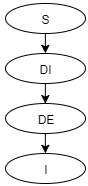
\includegraphics[width=2cm]{appStdNum}\\
  \caption{Graphical setup of determining student number.}
  \label{fig:stdNum}
\end{figure}

$DE$ is further described by 
\begin{align}
% \nonumber to remove numbering (before each equation)
  P(DE) =  P(BE_1,CE_1,BE_2,CE_2,...,BE_8,CE_8).
\label{eqn:ansIndep}
\end{align}

$DI$ is described by,

\begin{align}
% \nonumber to remove numbering (before each equation)
  P(DI) =  P(D_1,D_2,...,D_8).
\label{eqn:ansIndep2}
\end{align}

$P(S/DE)$ can now be represented by
\begin{align}
% \nonumber to remove numbering (before each equation)
  P(S/DE)	=  \sum_{\forall DI}^{}  P(S,DI/DE)\\
  					=  \sum_{\forall DI}^{}  \frac{P(BE/S,DI)P(S,DI)}{P(DE)}.
\label{eqn:stdEqn2}
\end{align}

In Equation \ref{eqn:stdEqn2}, the digit intended term, $DI$, is brought in by making use of the sum rule. Bayes' rule is then applied as shown.

In Figure \ref{fig:stdNum}, $DE$ is seen to be independent from $S$ if $DI$ is known and thus,

\begin{align}
% \nonumber to remove numbering (before each equation)
  P(S/DE)	=  \sum_{\forall DI}^{}  \frac{P(BE/DI)P(DI/S)P(S)}{P(DE)}.
\label{eqn:stdEqn3}
\end{align}

Finally from the digit and student number graph structure the following independence properties are also known,

\begin{align}
P(DE/ID) = P(BE_1/BI_1)P(CE/D_1)...P(BE_8/BI_8)P(CE/D_8)\\
\label{eqn:stdEqn4}
\end{align}

$P(S)$ can be initialized as an equal distribution, because every student number has the same likelihood in a given test. $P(DI/S)$ are values that are trained from data using the independence property, 
\begin{align}
P(DI/S) = P(D_1/S)...P(D_8/S).
\label{eqn:stdEqn4}
\end{align}
This value symbolizes the probability that the user intended to write down a digit given that student number. If the first digit of the student number is 1, the first intended digit will have a high probability of being 1. Thus these two random variables are strongly correlated. The only values that still need to be calculated are thus $P(DE/ID)$. Using the indepenency property of \begin{align}
P(DE/ID) = P(BE_1/BI_1)P(CE/D_1)...P(BE_8/BI_8)P(CE/D_8),
\label{eqn:stdEqn4}
\end{align}
the intended digit model's conditional distributions can be used. The two PGM models can now be fully defined and used to infer the intended student entries from an image. %Implementation/Algorithms
\chapter{Systems diagrams}
\label{ap:Algorithms}
\graphicspath{{Appendix4/Appendix4figures/}}

\section{Interface}

The software's main interface and clash list is show in Figure \ref{fig:mainInterface} and Figure \ref{fig:clashInterface}.

\begin{figure}
  \centering
  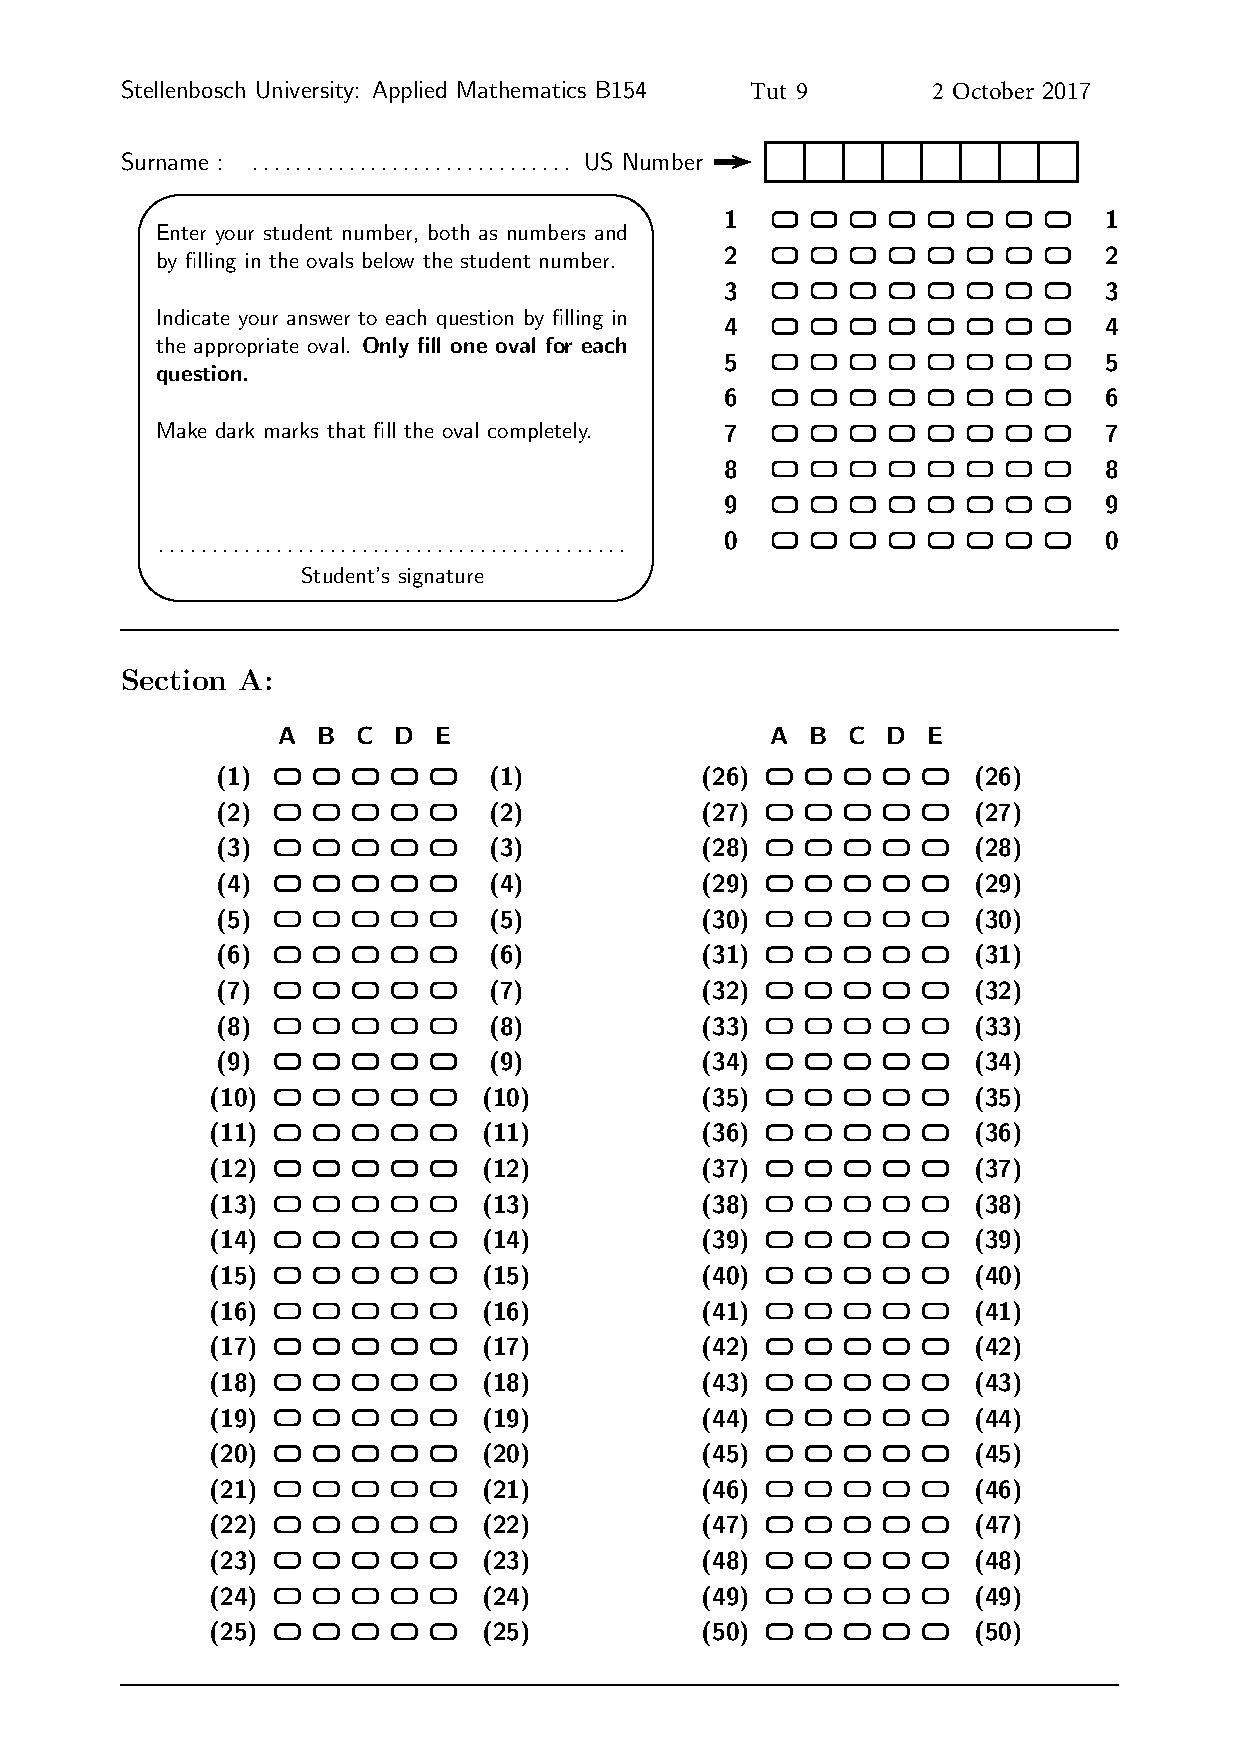
\includegraphics[width=14cm]{mainInterface}\\
  \caption{Main interface of test grader.}
  \label{fig:mainInterface}
\end{figure}

\begin{figure}
  \centering
  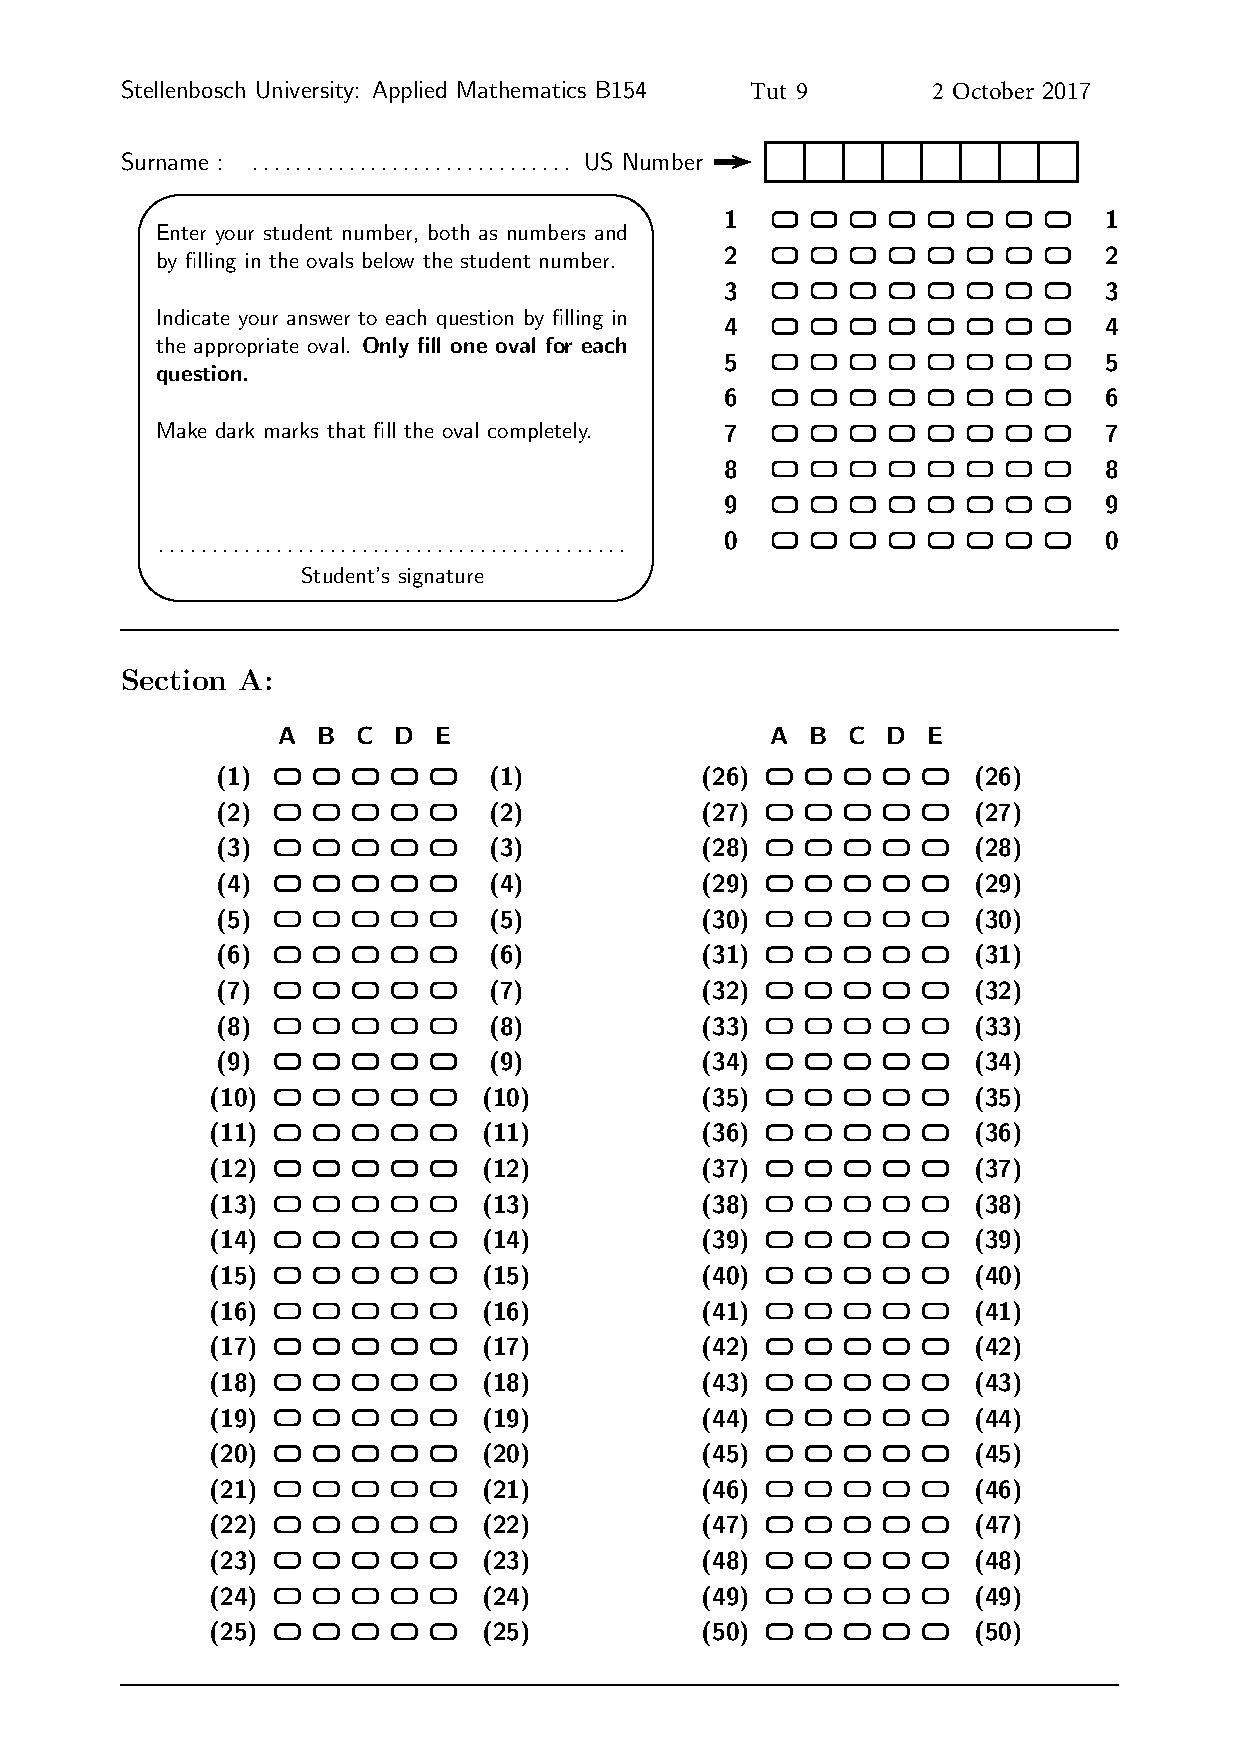
\includegraphics[width=14cm]{clashInterface}\\
  \caption{Clash list interface of test grader.}
  \label{fig:clashInterface}
\end{figure}

\section{Templates}

The original template can be seen in the Figures \ref{fig:template1}. 

\begin{figure}
  \centering
  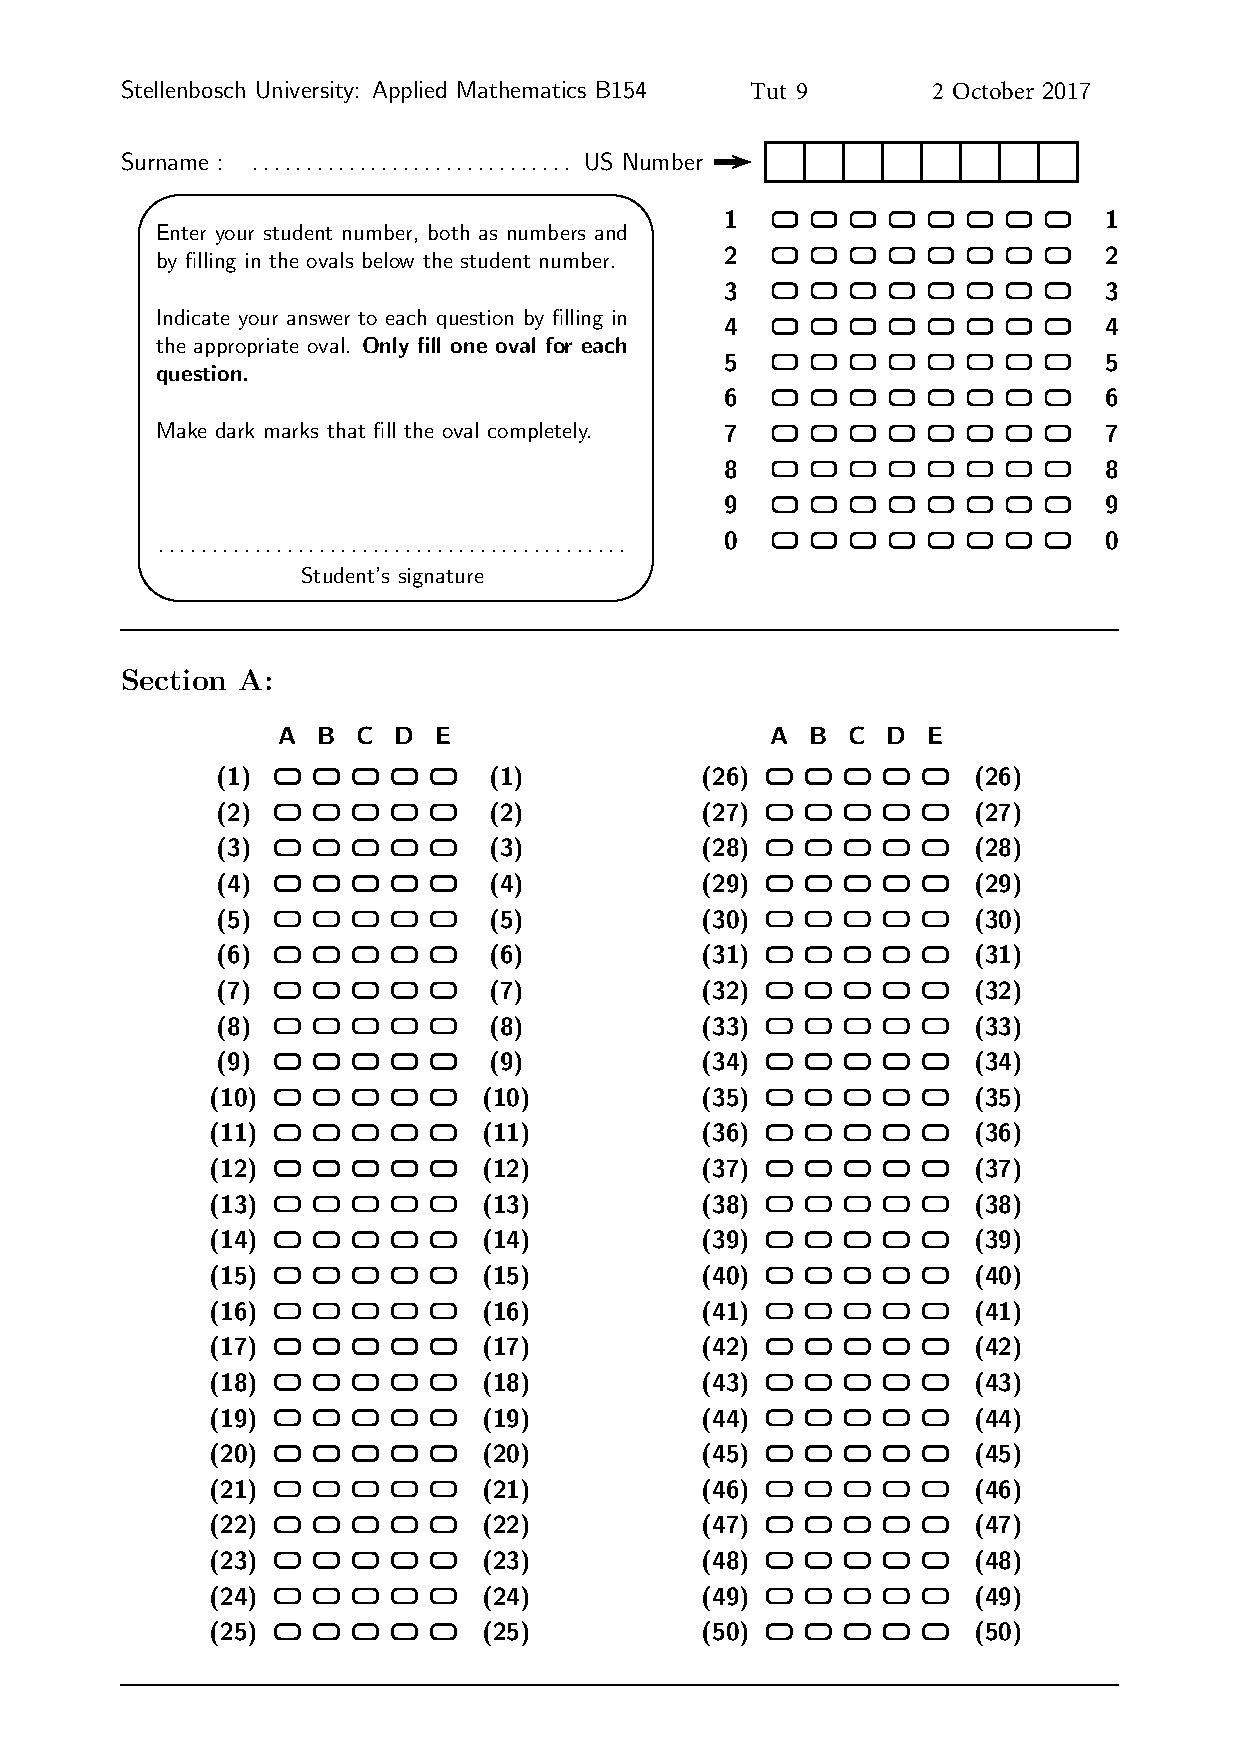
\includegraphics[width=12cm]{template1}\\
  \caption{Original template focussed on numbered answered questions.}
  \label{fig:template1}
\end{figure}

Two additional templates has also been developed and implemented for the department. These templates gives the department the capabilities of grading numbered answered questions as well as multiple choice questions. These templates are shown in Figure \ref{fig:template2} and Figure \ref{fig:template3}.

\begin{figure}
  \centering
  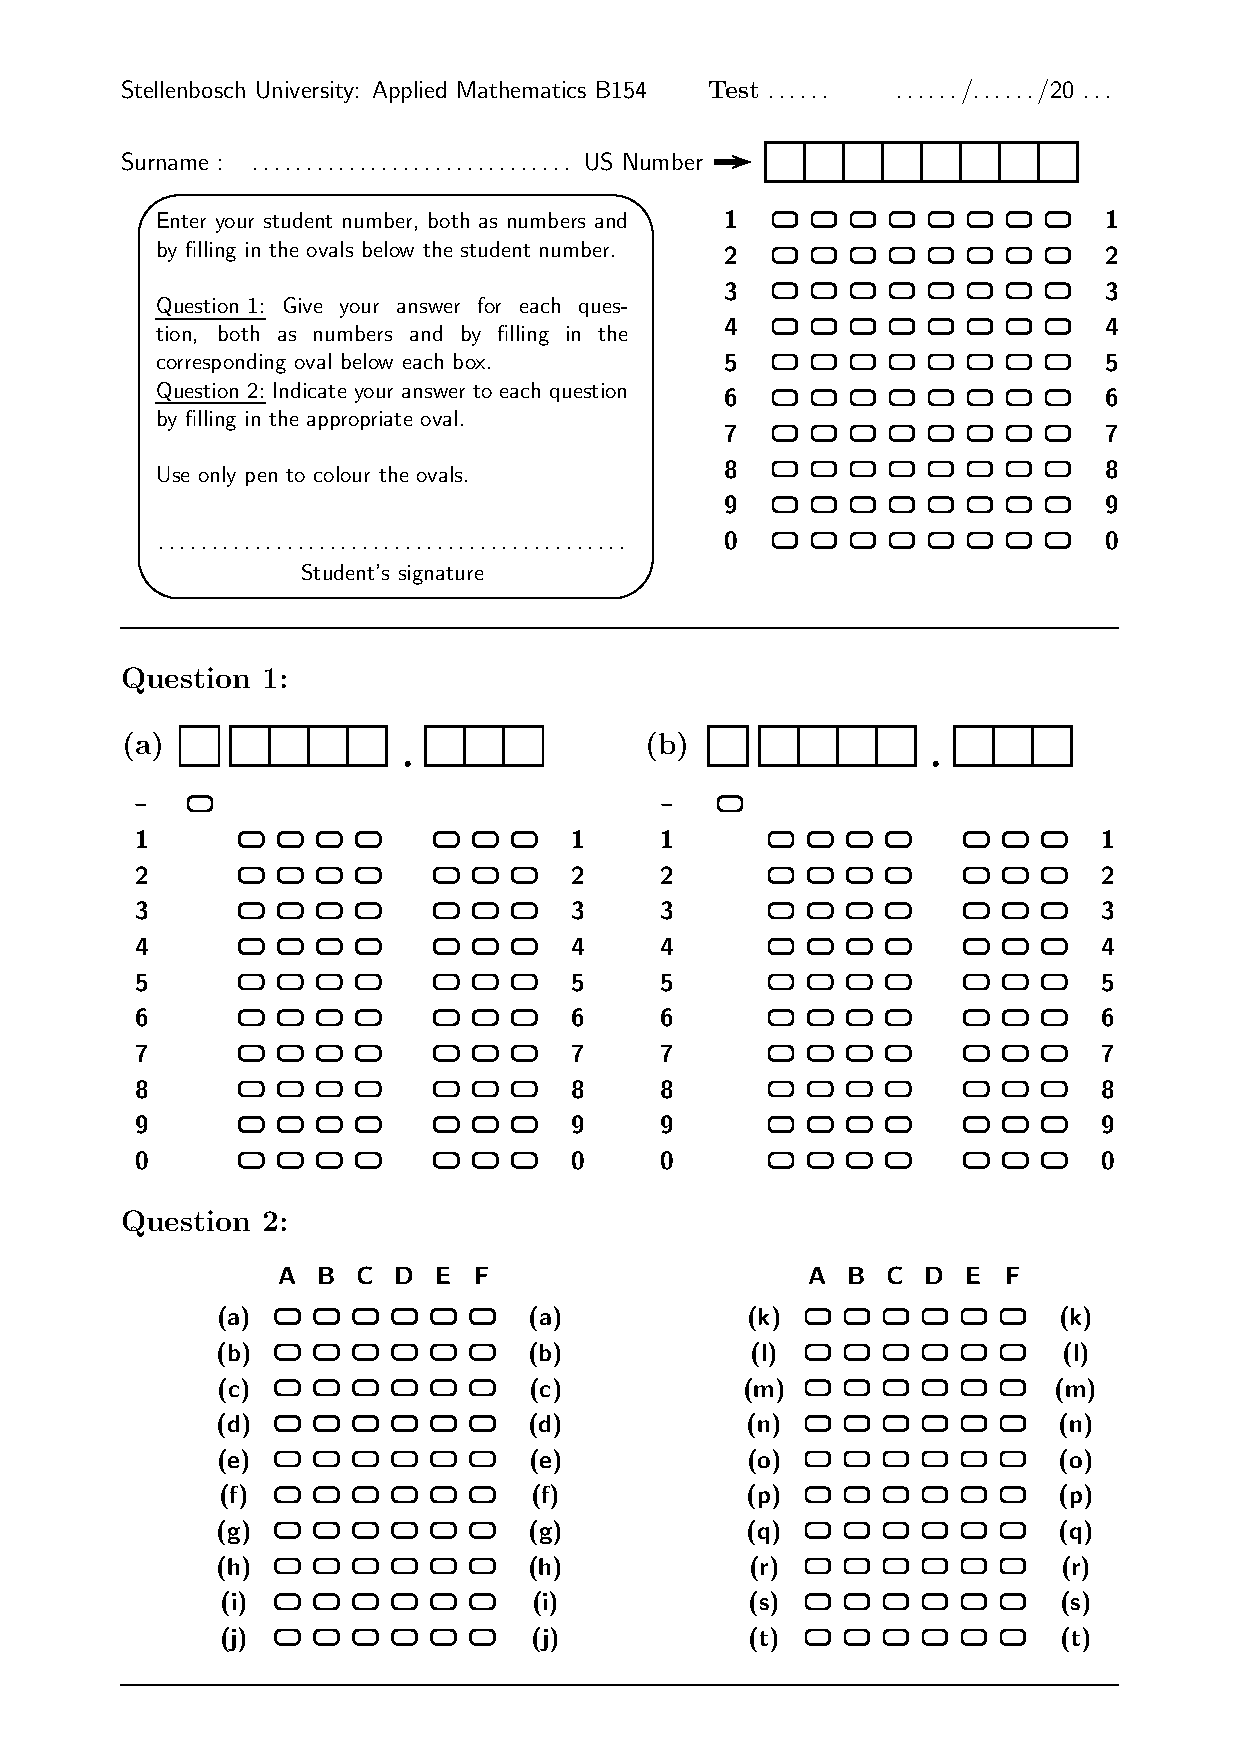
\includegraphics[width=12cm]{template2}\\
  \caption{Template allowing for numbered and multiple choice answers.}
  \label{fig:template2}
\end{figure}

\begin{figure}
  \centering
  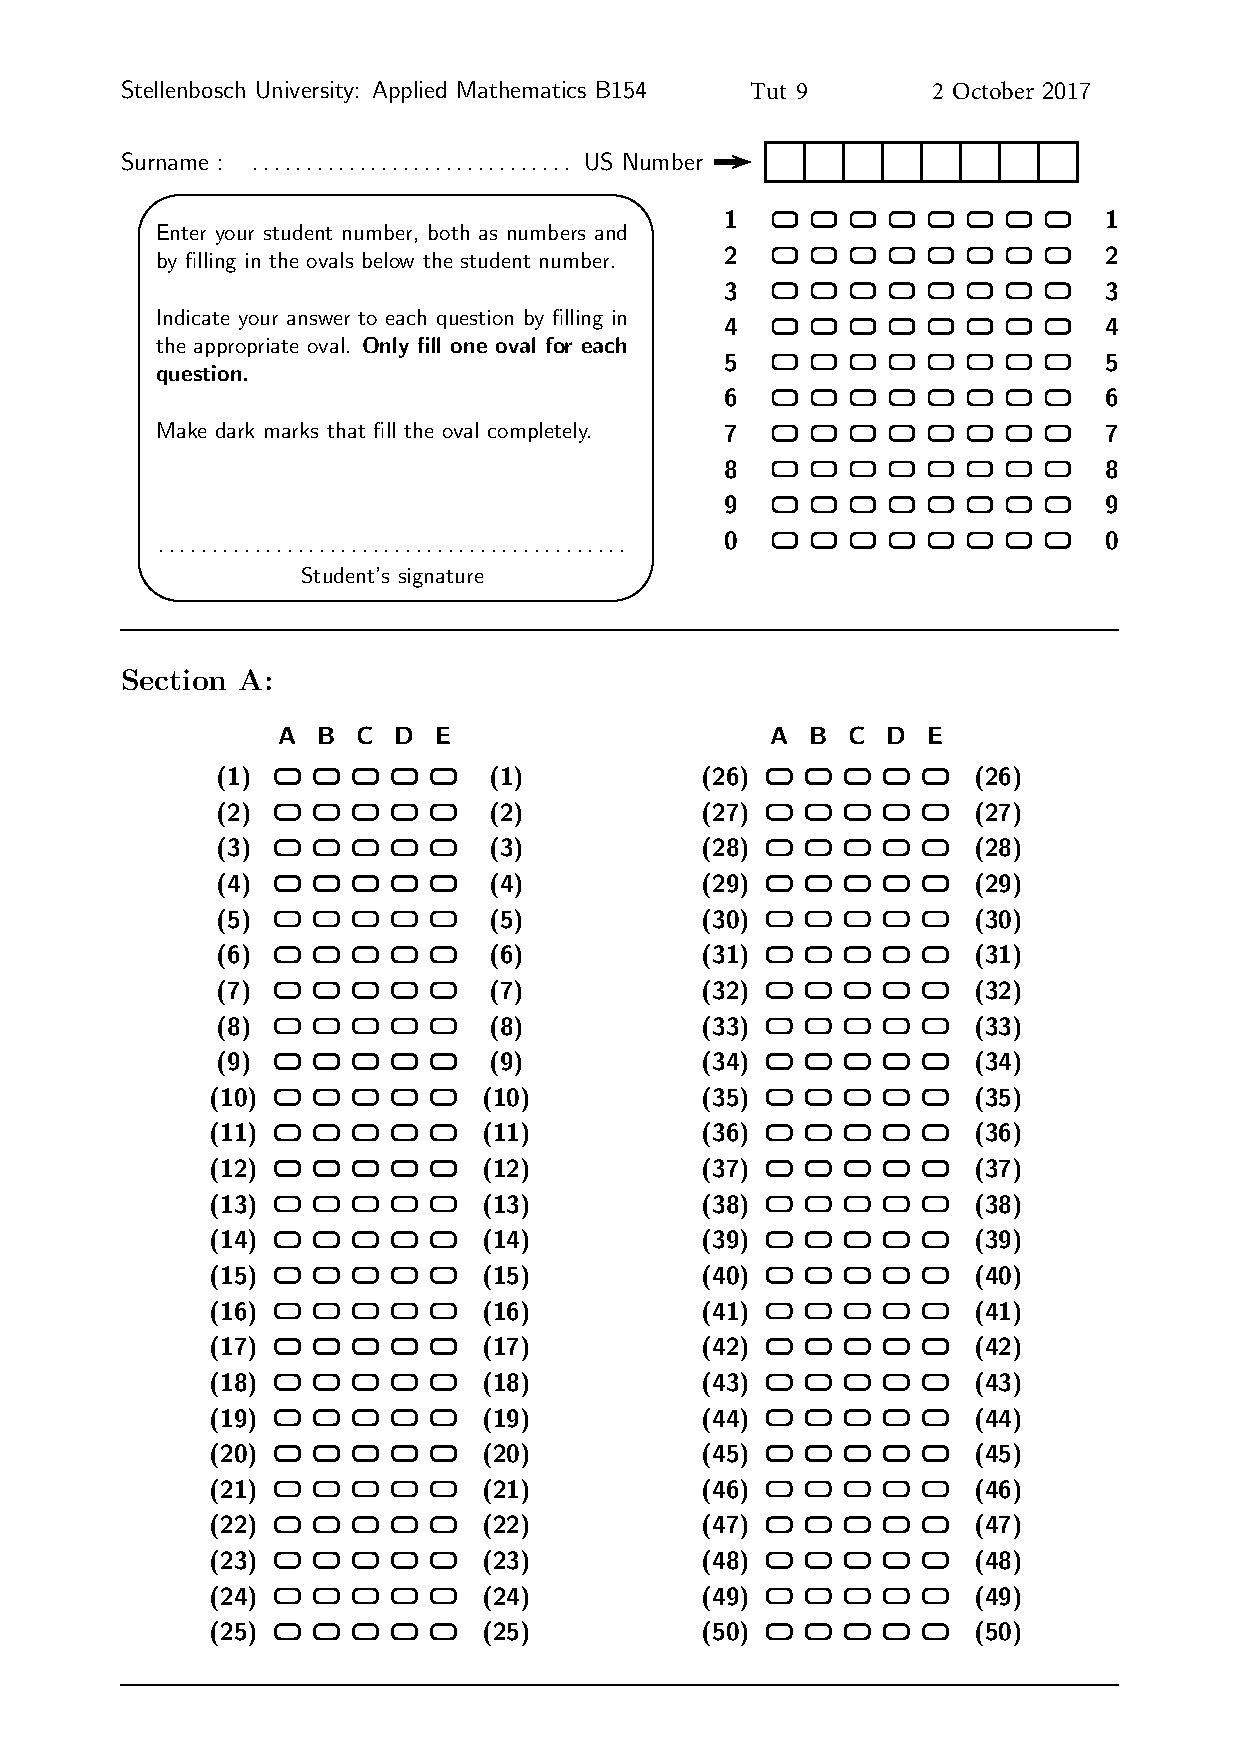
\includegraphics[width=12cm]{template3}\\
  \caption{Template focussed just on multiple choice type questions.}
  \label{fig:template3}
\end{figure}

\section{DCNN TensorFlow setup}
The DCNN structural setup diagram can be seen in Figure \ref{fig:DCNN}. This structure was directly used as constructed was constructed by the TensorFlow team.

\begin{figure}
  \centering
  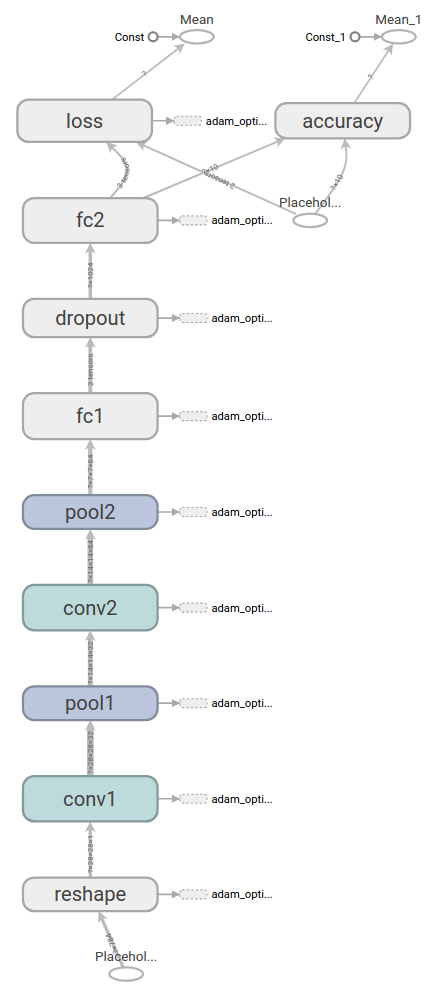
\includegraphics[width=7cm]{DCNN}\\
  \caption{DCNN structural setup diagram, from \citet{Tensor}}
  \label{fig:DCNN}
\end{figure} %Results and validation
\chapter{Validation and results}
\label{ap:results}
\graphicspath{{Appendix5/Appendix5figures/}}

This appendix described additional test results obtained from experiments done on the systems.

\section{All tutorial results}
\label{sec:tutorialResults}

\subsection{Overview}

This automatic test grader was sucesfully used to grade 11 tutorial test in 2017. In that 11 tutorial an approximately of 99.6\% of test was graded correctly, as no corrections were made by students. The ta

\begin{table}
\caption{Description of tutorial results.} \label{tbl:tutResults}
  \centering
\begin{tabular}{|p{3cm}|p{3cm}|p{5cm}|}
\hline
\textbf{Tutorial number}&\textbf{Number of tests graded incorrectly}&\textbf{Reason for results}\\
\hline
\multicolumn{3}{|l|}{Basic system is now implemented.}\\
\hline
Tutorial 1&3&Hello assdafsadfsa dfsdfsdafdsf asdfsadfasdf sadfasdfa sdfsadfs adfasdfs dfasdfsdafsa dfsdf sadfasdf asdf asdfa dfasd fsad fsad fsa dfsdf.\\
\hline
Tutorial 2&3&Hello assdafsadfsa dfsdfsdafdsf asdfsadfasdf sadfasdfa sdfsadfs adfasdfs dfasdfsdafsa dfsdf sadfasdf asdf asdfa dfasd fsad fsad fsa dfsdf.\\
\hline
Tutorial 3&3&Hello assdafsadfsa dfsdfsdafdsf asdfsadfasdf sadfasdfa sdfsadfs adfasdfs dfasdfsdafsa dfsdf sadfasdf asdf asdfa dfasd fsad fsad fsa dfsdf.\\
\hline
Tutorial 4&3&Hello assdafsadfsa dfsdfsdafdsf asdfsadfasdf sadfasdfa sdfsadfs adfasdfs dfasdfsdafsa dfsdf sadfasdf asdf asdfa dfasd fsad fsad fsa dfsdf.\\
\hline
Tutorial 5&3&Hello assdafsadfsa dfsdfsdafdsf asdfsadfasdf sadfasdfa sdfsadfs adfasdfs dfasdfsdafsa dfsdf sadfasdf asdf asdfa dfasd fsad fsad fsa dfsdf.\\
\hline
Tutorial 6&3&Hello assdafsadfsa dfsdfsdafdsf asdfsadfasdf sadfasdfa sdfsadfs adfasdfs dfasdfsdafsa dfsdf sadfasdf asdf asdfa dfasd fsad fsad fsa dfsdf.\\
\hline
\end{tabular} 
\end{table}

\begin{table}
\caption{Description of tutorial results.} \label{tbl:tutResults2}
  \centering
\begin{tabular}{|p{3cm}|p{3cm}|p{5cm}|}
\hline
\multicolumn{3}{|l|}{Compete system is now implemented.}\\
\hline
Tutorial 7&3&Hello assdafsadfsa dfsdfsdafdsf asdfsadfasdf sadfasdfa sdfsadfs adfasdfs dfasdfsdafsa dfsdf sadfasdf asdf asdfa dfasd fsad fsad fsa dfsdf.\\
\hline
Tutorial 8&3&Hello assdafsadfsa dfsdfsdafdsf asdfsadfasdf sadfasdfa sdfsadfs adfasdfs dfasdfsdafsa dfsdf sadfasdf asdf asdfa dfasd fsad fsad fsa dfsdf.\\
\hline
Tutorial 9&3&Hello assdafsadfsa dfsdfsdafdsf asdfsadfasdf sadfasdfa sdfsadfs adfasdfs dfasdfsdafsa dfsdf sadfasdf asdf asdfa dfasd fsad fsad fsa dfsdf.\\
\hline
Tutorial 10&3&Hello assdafsadfsa dfsdfsdafdsf asdfsadfasdf sadfasdfa sdfsadfs adfasdfs dfasdfsdafsa dfsdf sadfasdf asdf asdfa dfasd fsad fsad fsa dfsdf.\\
\hline
Tutorial 11&3&Hello assdafsadfsa dfsdfsdafdsf asdfsadfasdf sadfasdfa sdfsadfs adfasdfs dfasdfsdafsa dfsdf sadfasdf asdf asdfa dfasd fsad fsad fsa dfsdf.\\
\hline
\end{tabular}
\end{table}
\section{Deep Convolutional Neural Network test results}
\label{sec:DCNNresult}

This section describes the results obtained on testing a trained neural network on a test dataset. Tests is conducted on 3 neural networks trained on different datasets and compared with each other. This testing proses is conducted to find the neural network weights that will classified had written digits the most accurately. The neural networks is tested on a test dataset generated by grading 900 student tests, while extracting the character images. The answers from these tests is used to create labels for each digit image. Thus each 28 by 28 pixel digit image has a accompanied label specifies what that digit is. The database contains 16 000 labelled images. An additional dataset, called the MNIST dataset was also used in this proses. This dataset contains 60 000 images 
\section{Trained on generated database}
For a first attempt at training the neural network 10 000 of the generated database is used. The remaining 6000 digits is then used to test the accuracy of the network.

\subsection{Accuracy of network}

\subsection{Conclusion on accuracy}

\section{Trained on MNIST database}
For a first attempt at training the neural network 10 000 of the generated database is used. The remaining 6000 digits is then used to test the accuracy of the network.

\subsection{Accuracy of network}

\subsection{Conclusion on accuracy}


\section{Trained on mixed database}
For a first attempt at training the neural network 10 000 of the generated database is used. The remaining 6000 digits is then used to test the accuracy of the network.

\subsection{Accuracy of network}

\subsection{Conclusion on accuracy}











Attempt 2:

Accuracy for character recognition:

Using default deep neural network. V23

Test accuracy for network trained on MNIST dataset:
On test data for MNIST: 		0.9935
On test data for generated digits: 	0.666667

Main reason for error.
The MNIST dataset has images that are more consentrated to being binary.
Either black or white.

Test accuracy for network trained on generated digits:
On test data for MNIST:			 0.9462
On test data for generated digits:	 0.921569


Reasons The algorithm above does not work that well on the characters:

Accuracy for character recognition:

Using default deep neural network. Up to V22

Test accuracy for network trained on MNIST dataset:
On test data for MNIST: 		0.9935
On test data for generated digits: 	0.666667

Main reason for error.
The MNIST dataset has images that are more consentrated to being binary.
Either black or white.

Test accuracy for network trained on generated digits:
On test data for MNIST:			 0.9462
On test data for generated digits:	 0.921569


Reasons The algorithm above does not work that well on the characters:


Borders are not cut out properly.

Neural network focusses on color as well which decreases its accuracty for shape.
 %ProjectPlan


%\include{Appendix7/appendix7} %Experiments

%\chapter{Mathematical and graphical description of system}
\label{ap:systemOverview}
\graphicspath{{Appendix3/Appendix3Figures/},{Chapter1/Chapter1Figures/},{Chapter4/Chapter4Figures/}}

In this appendix a graphical and mathematical derivation for the system is given. It is shown through mathematical derivation how the pgmpy software can predict the student number and answer given the probability distributions and evidence. It should be noted that the software exploits additional methods in calculating these values in an efficient manner.

\section{High-level overview}

\begin{figure}
  \centering
  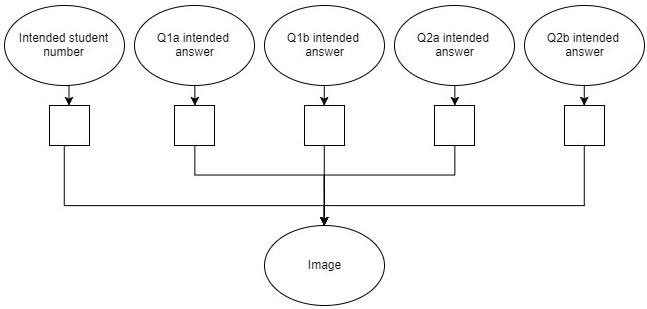
\includegraphics[width=11cm]{systemOverview}\\
  \caption{System overview.}
  \label{fig:appOverview}
\end{figure}
\nomenclature[S]{$A$}{Random variable representing an answer for a specific question}
\nomenclature[S]{$I$}{Random variable representing the test image}
\nomenclature[S]{$S$}{Random variable representing the possible student number}
As described in Chapter \ref{ch:Introduction}, the system can fundamentally be represented with 6 information nodes. These nodes are shown in Figure \ref{fig:appOverview}. The student has 5 pieces of information that he/she wants to portray, signifying the first 5 nodes. Those 5 nodes give rise to the image, representing the last node. At its core the system is tasked with inferring two types of conditional probabilities namely $P(S/I)$ and $P(A/I)$. The random variables $S$ and $A$ represent all the possible values that the student number and answers can possibly have. The image, $I$, is also a random variable representing the total number of possible states the image can take. Each image has a width and length of 1 240 by 1 754 pixels. For every pixel there are 256 possible values, ranging from 0.0 to 1.0. Thus the number of possible images are in the range of 1 240 $\times$ 1 754 $\times$ 256. To practically represent this, more detailed derivations and assumptions is needed. These derivations are described in the next sections. 
 
%The aim of the software is to maximize the likelihood of those probability distributions indicating the correct answers.
%The reason the problem is represented in a probabilistic way is due to the fact that different images are going to be generated every time a test is written. This is true even when the same information is going to be portrayed. Everytime a student writes a test he/she is going to write in different ways. A probabilistic graphical model (PGM) is thus used to describe this system and its inner operations. For a more detailed explanation on PGM's, refer to Section \ref{sec:PGM}.  The blocks in Figure \ref{fig:systemOverview} represent additional processing that is described in the following sections.

\section{The student answer}
In Section \ref{sec:studentAnswer}, it was determined that the student's answer can be calculated by combining the intended sign and digits of each column separately. This is attributed to the fact that these digits are independent of one another, as seen in Figure \ref{fig:appAns}. 

\begin{figure}
  \centering
  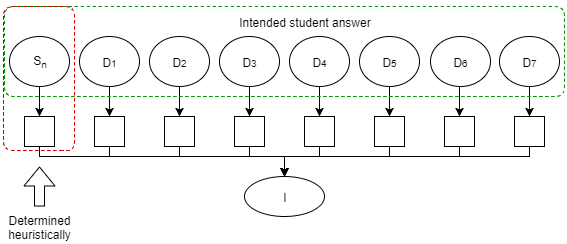
\includegraphics[width=10cm]{appAns}\\
  \caption{Graphical setup of determining student answer.}
  \label{fig:appAns}
\end{figure}
\nomenclature[S]{$Sn$}{Random variable representing the sign of a specific answer}
\nomenclature[S]{$D_i$}{Random variable representing a digit in column $i$ for a answer or student number block}
The intended digit in a certain column is not influenced by what the values in the other columns are. This independence property is thus described by\begin{align}
% \nonumber to remove numbering (before each equation)
  P(A/I) =  P(Si/I)P(D_1/I)...P(D_7/I),
\label{eqn:ansIndep}
\end{align}
where $A$ and $I$ again represent an answer  for a specific question and the image, respectively. The random variable $Si$ represents the sign of the answer.

To find the most probable answer, only $P(Sn/I)$ and $P(D_{1-7}/I)$ need to be calculated. Using image processing techniques described in Section \ref{ch:ImageProcessing}, $P(Si/I)$ can simply be determined heuristically by determining the probability of the bubble being coloured in, underneath the sign. Thus the only values yet to calculate is $P(D_{1-7}/I)$ and derived in the next section.

\section{The intended digit}

\begin{figure}
  \centering
  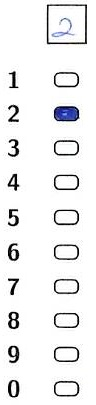
\includegraphics[width=1cm]{column}\\
  \caption{Column with evidence that gets considered for the calculation of an intended digit.}
  \label{fig:column}
\end{figure}

In determining an intended digit there are 11 information nodes to use as evidence. These nodes represent the 10 bubbles and character block, as shown in Figure \ref{fig:column}. Extra nodes are also added to symbolise the intended bubbles as described in Section \ref{sec:studentDigit}. The first bubble might sometimes incorrectly be associated with digit 0. Thus even if the student intended the digit 0 as an answer, the intended bubble of that student was actually the bubble for digit 1.

\begin{figure}
  \centering
  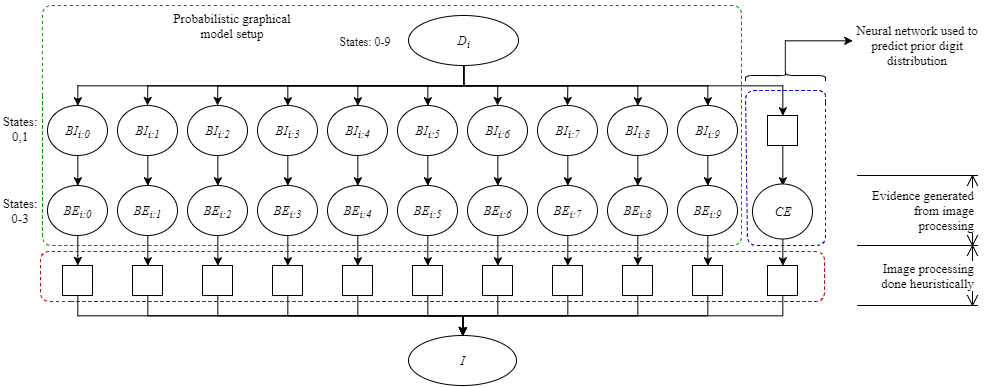
\includegraphics[width=16cm]{appDigit}\\
  \caption{Graphical setup of determining intended digit.}
  \label{fig:appDigit}
\end{figure}
\nomenclature[S]{$BE_i$}{Random variable representing bubble evidence obtained form image processing of the digit at index $i$}
\nomenclature[S]{$CE_i$}{Random variable representing a character evidence obtained form image processing at and arbitrary index $i$}

The probability of each column's digit is describe by $P(D_i/I)$. This value represents the probability of each of the 10 digits being written down in column $i$ . We know that the digit evidence is calculated heuristically using image processing. Each bubble thus has an evidence value with 4 possible states, namely not filled-in, crossed out, partially filled-in and completely filled-in. Thus the estimate of the intended digit is now represented by $P(D_i/I,BE_i,CE_i)$. $BE_i$ and $CE_i$ represents all the bubble and character evidence for that digit. As seen in Figure \ref{fig:appDigit}, $D_i$ and $I$ becomes independent from one another given the values of $BE_i$ and $CE_i$. Thus the probability of the intended digit is now given by $P(D_i/BE_i,CE_i)$.
\nomenclature[S]{$BI_i$}{Random variable representing the bubbles the student to colour in for digit $i$}
$BE_i$ is further described by 
\begin{align}
% \nonumber to remove numbering (before each equation)
  P(BE_i) =  P(BE_{i:0},BE_{i:1},...,BE_{i:9}),
\label{eqn:ansIndep}
\end{align}
where  $P(BE_{i:j})$ represents the digit i at bubble j. $BI_i$ is then represented by
\begin{align}
% \nonumber to remove numbering (before each equation)
  P(BI_i) =  P(BI_{i:0},BI_{i:1},...,BI_{i:9}),
\label{eqn:ansIndep}
\end{align}
where  $P(BI_{i:j})$ represents the digit i at bubble j.

$P(D_i/BE_i,CE_i)$ can now be represented by
\begin{align}
% \nonumber to remove numbering (before each equation)
  P(D_i/BE_i,CE_i)	=  \sum_{\forall BI_i}^{}  P(D_i,BI_i/BE_i,CE_i)\\
  					=  \sum_{\forall BI_i}^{}  \frac{P(BE_i,CE_i/D_i,BI_i)P(D_i,BI_i)}{P(BE_i,CE_i)}.
\label{eqn:ansEqn2}
\end{align}

In Equation \ref{eqn:ansEqn2}, the intended bubble term is brought in by making use of the sum rule. Bayes' rule is then applied. In Figure \ref{fig:appDigit}, $BE_i$ and $CE_i$ is seen to be independent when $D_i$ or $BI_i$ is known. Further it is observed that $BE_i$ is only reliant on $BI_i$ and $CE_i$ on $D_i$. Thus by applying an additional product rule it is determined that
\begin{align}
  P(D_i/BE_i,CE_i) =  \sum_{\forall BI_i}^{}\frac{P(BE_i/BI_i)P(BI_i/D_i)P(CE_i/D_i)P(D_i)}{P(BE_i,CE_i)}.
\label{eqn:ansEqn3}
\end{align}

Bayes' rule also provides us with,
\begin{align}
  P(CE_i/D_i)	=  \frac{P(D_i/CE_i)PCE_i)}{P(D_i)}.
\label{eqn:ansEqn4}
\end{align}

Now by factoring out all the constant terms out of the summation the equation reduces to,
\begin{align}
  P(D_i/BE_i,CE_i) =  \frac{P(CE_i)}{P(BE_i,CE,i)}\sum_{\forall BI_i}^{}P(BE_i/BI_i)P(BI_i/D_i)P(D_i/CE_i).
\label{eqn:ansEqn5}
\end{align}
The constant terms gets ignored in the pgmpy package due to them only being normalizing terms. Once the summation has been calculated the software simply normalizes the resulting values without needing those terms. Thus only $P(BE_i/BI_i)$, $P(BI_i/D_i)$ and $P(D_i/CE_i)$ are needed.

$P(BE_i/BI_i)$ and  $P(BI_i/D_i)$ are both terms that is deduced from training. The final term that is needed is $P(D_i/CE_i)$. This term is efficiently represented through the use of a neural network. Thus the PGM system can successfully infer the digit probabilities and thus the student answer with these 3 distributions specified. A derivation on the student number probability is discussed next.

\section{The student number}
\nomenclature[S]{$DE$}{Random variables representing a digit evidence obtained form image processing}
\nomenclature[S]{$DI$}{Random variables all the digit intended by the student}
As state in Section \ref{sec:studentNumber}, the assumption of independence between digits does not hold in the case of a student number. The reason for this is, because every 8 digit number is not equally likely to be a student number. Only student numbers that are valid needs to be considered as a possible state that the student number node can take. This node has approximately $900$ states, depending on the number of student numbers. The student number graph can be seen in Figure \ref{fig:stdNum}. 

A derivation for $P(S/I)$ is needed next. As stated previously, $S$ represents a random variable over all the possible student numbers. $I$ again represents the image. We know that the digit evidence is calculated heuristically using image processing. Thus the estimate of the student number is now represented as $P(S/I,DE)$. $DE$ now represents all the bubble and character evidence. As seen in Figure \ref{fig:stdNum}, $S$ and $I$ becomes independent from one another given the values of $DE$. Thus the probability of the intended digit is now given by $P(S/DE)$.

\begin{figure}
  \centering
  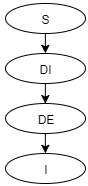
\includegraphics[width=2cm]{appStdNum}\\
  \caption{Graphical setup of determining student number.}
  \label{fig:stdNum}
\end{figure}

$DE$ is further described by 
\begin{align}
% \nonumber to remove numbering (before each equation)
  P(DE) =  P(BE_1,CE_1,BE_2,CE_2,...,BE_8,CE_8).
\label{eqn:ansIndep}
\end{align}

$DI$ is described by,

\begin{align}
% \nonumber to remove numbering (before each equation)
  P(DI) =  P(D_1,D_2,...,D_8).
\label{eqn:ansIndep2}
\end{align}

$P(S/DE)$ can now be represented by
\begin{align}
% \nonumber to remove numbering (before each equation)
  P(S/DE)	=  \sum_{\forall DI}^{}  P(S,DI/DE)\\
  					=  \sum_{\forall DI}^{}  \frac{P(BE/S,DI)P(S,DI)}{P(DE)}.
\label{eqn:stdEqn2}
\end{align}

In Equation \ref{eqn:stdEqn2}, the digit intended term, $DI$, is brought in by making use of the sum rule. Bayes' rule is then applied as shown.

In Figure \ref{fig:stdNum}, $DE$ is seen to be independent from $S$ if $DI$ is known and thus,

\begin{align}
% \nonumber to remove numbering (before each equation)
  P(S/DE)	=  \sum_{\forall DI}^{}  \frac{P(BE/DI)P(DI/S)P(S)}{P(DE)}.
\label{eqn:stdEqn3}
\end{align}

Finally from the digit and student number graph structure the following independence properties are also known,

\begin{align}
P(DE/ID) = P(BE_1/BI_1)P(CE/D_1)...P(BE_8/BI_8)P(CE/D_8)\\
\label{eqn:stdEqn4}
\end{align}

$P(S)$ can be initialized as an equal distribution, because every student number has the same likelihood in a given test. $P(DI/S)$ are values that are trained from data using the independence property, 
\begin{align}
P(DI/S) = P(D_1/S)...P(D_8/S).
\label{eqn:stdEqn4}
\end{align}
This value symbolizes the probability that the user intended to write down a digit given that student number. If the first digit of the student number is 1, the first intended digit will have a high probability of being 1. Thus these two random variables are strongly correlated. The only values that still need to be calculated are thus $P(DE/ID)$. Using the indepenency property of \begin{align}
P(DE/ID) = P(BE_1/BI_1)P(CE/D_1)...P(BE_8/BI_8)P(CE/D_8),
\label{eqn:stdEqn4}
\end{align}
the intended digit model's conditional distributions can be used. The two PGM models can now be fully defined and used to infer the intended student entries from an image. %DelynoMinutes
%\chapter{Systems diagrams}
\label{ap:Algorithms}
\graphicspath{{Appendix4/Appendix4figures/}}

\section{Interface}

The software's main interface and clash list is show in Figure \ref{fig:mainInterface} and Figure \ref{fig:clashInterface}.

\begin{figure}
  \centering
  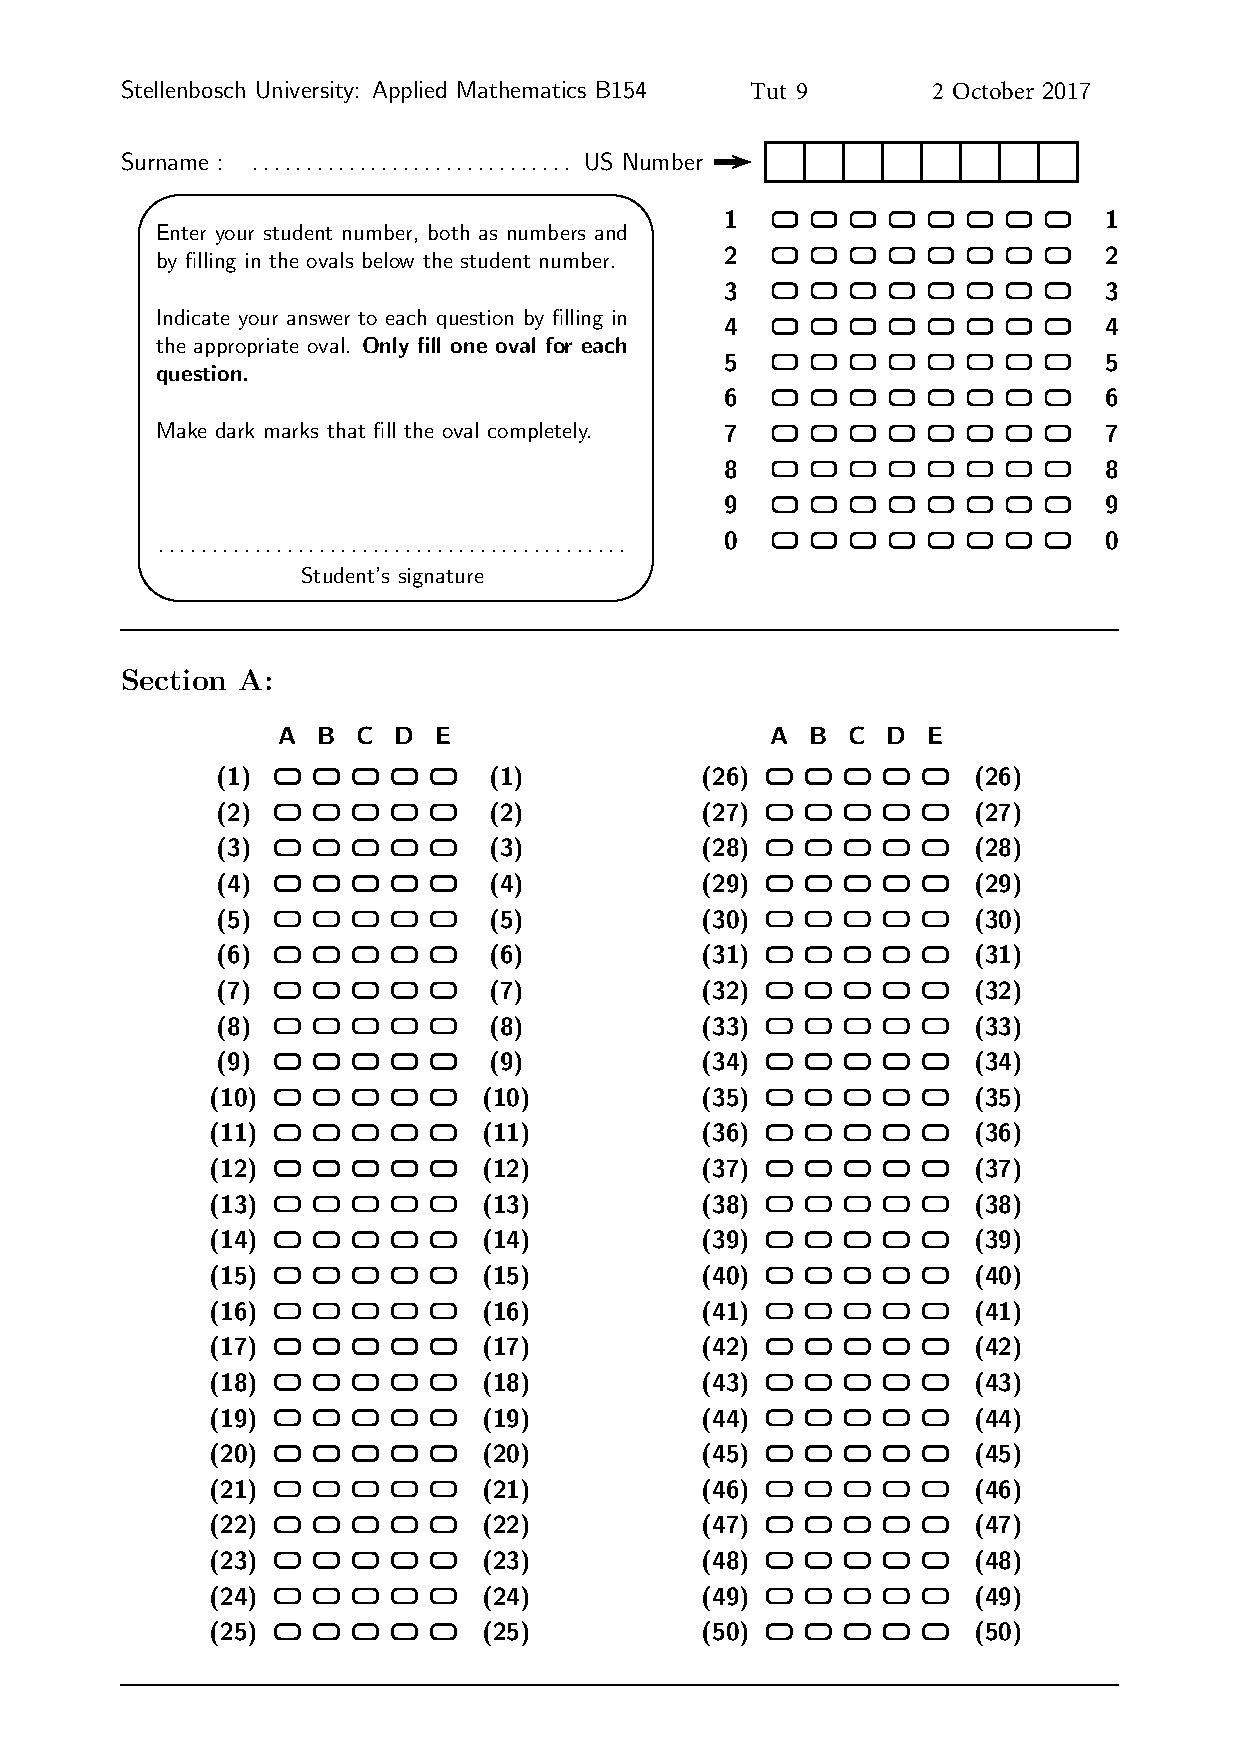
\includegraphics[width=14cm]{mainInterface}\\
  \caption{Main interface of test grader.}
  \label{fig:mainInterface}
\end{figure}

\begin{figure}
  \centering
  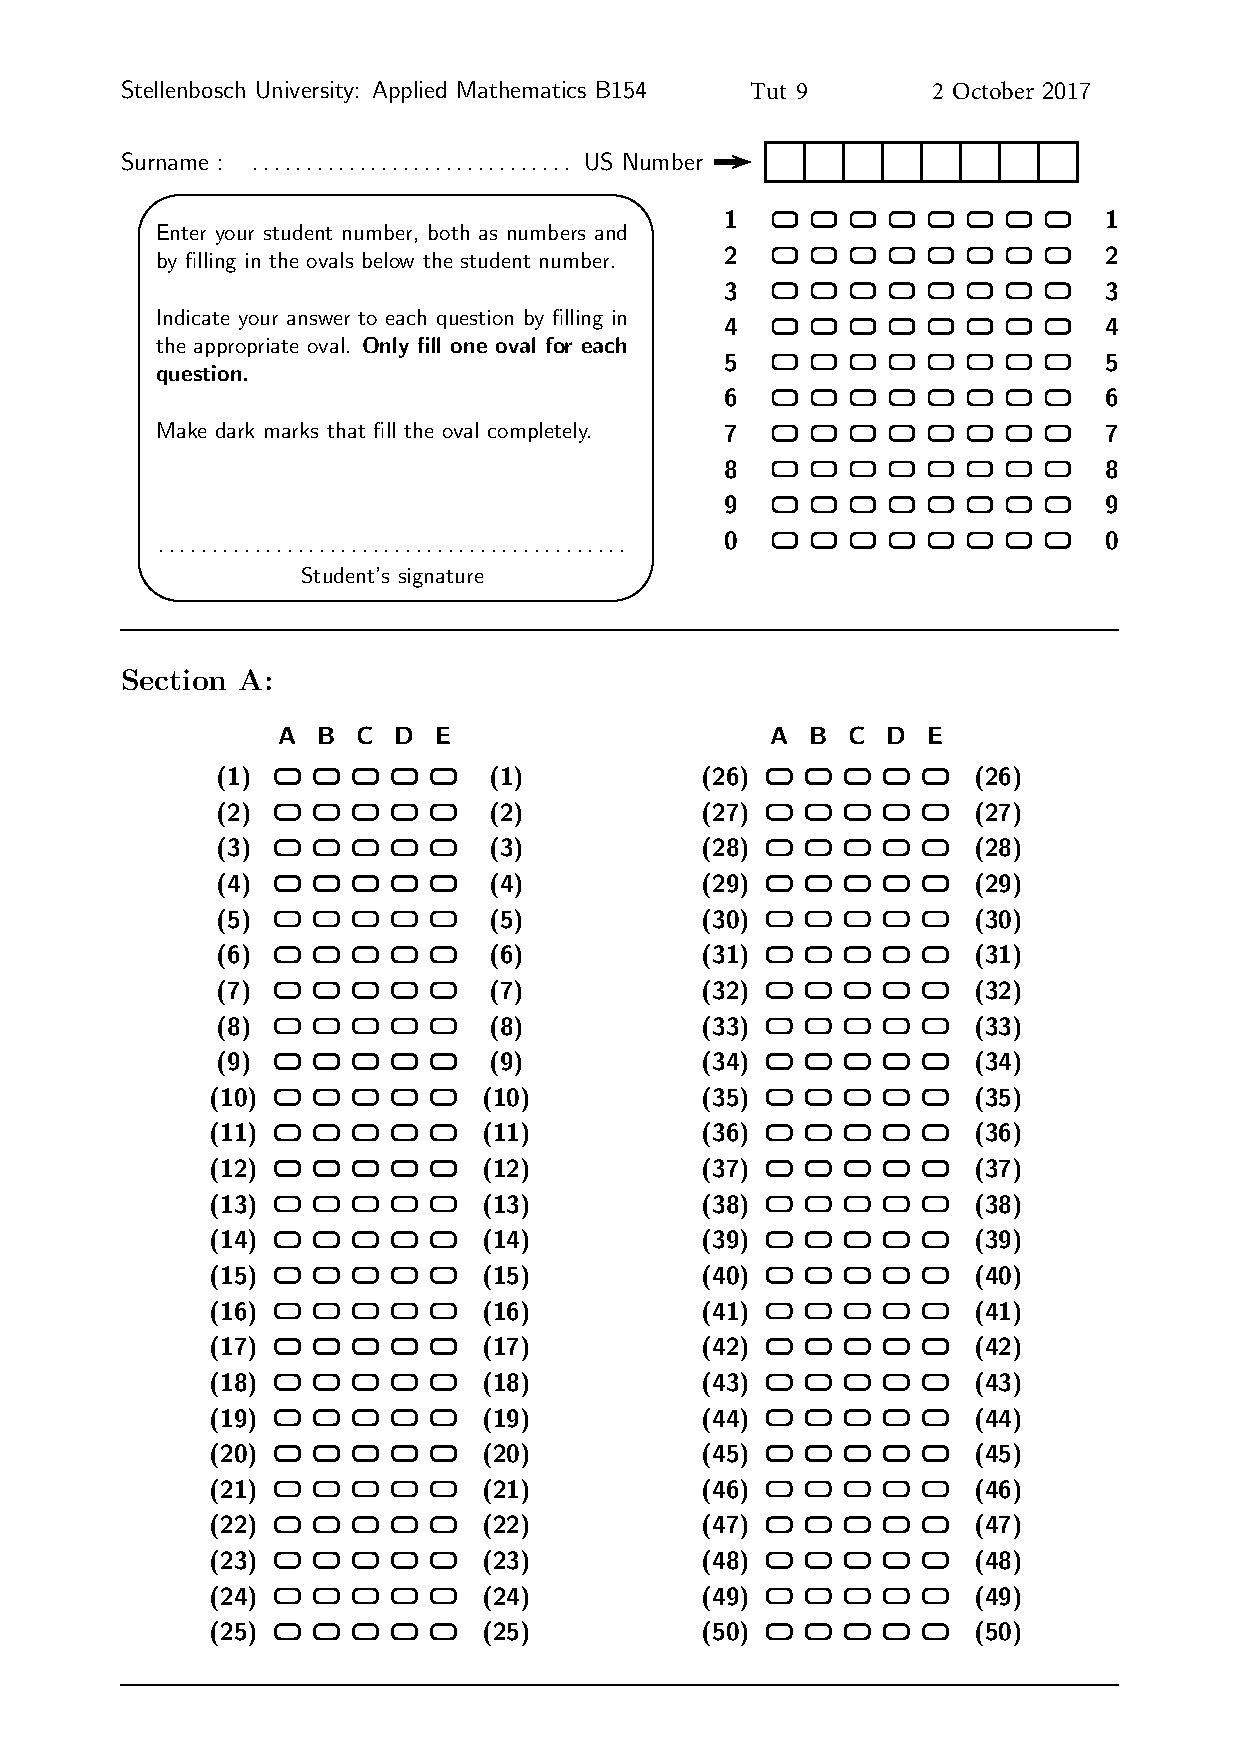
\includegraphics[width=14cm]{clashInterface}\\
  \caption{Clash list interface of test grader.}
  \label{fig:clashInterface}
\end{figure}

\section{Templates}

The original template can be seen in the Figures \ref{fig:template1}. 

\begin{figure}
  \centering
  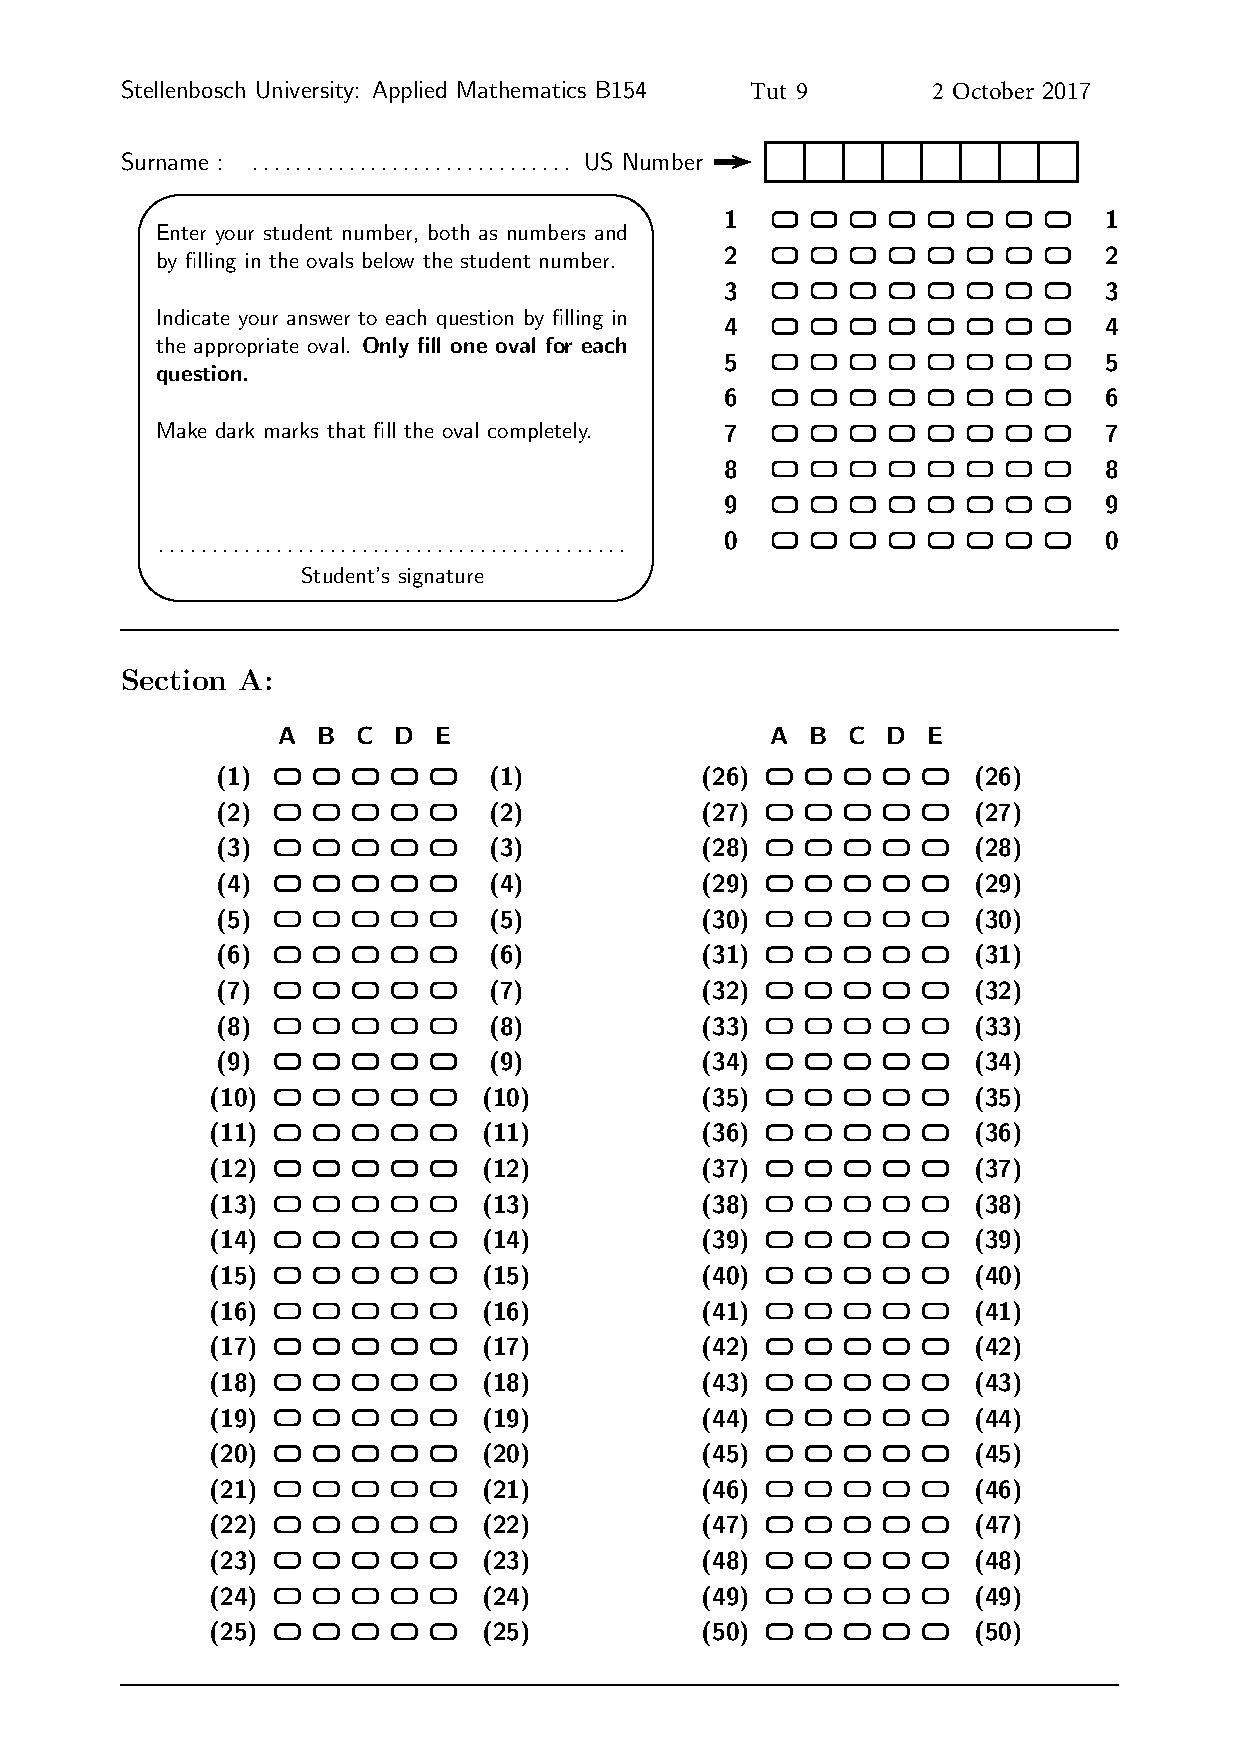
\includegraphics[width=12cm]{template1}\\
  \caption{Original template focussed on numbered answered questions.}
  \label{fig:template1}
\end{figure}

Two additional templates has also been developed and implemented for the department. These templates gives the department the capabilities of grading numbered answered questions as well as multiple choice questions. These templates are shown in Figure \ref{fig:template2} and Figure \ref{fig:template3}.

\begin{figure}
  \centering
  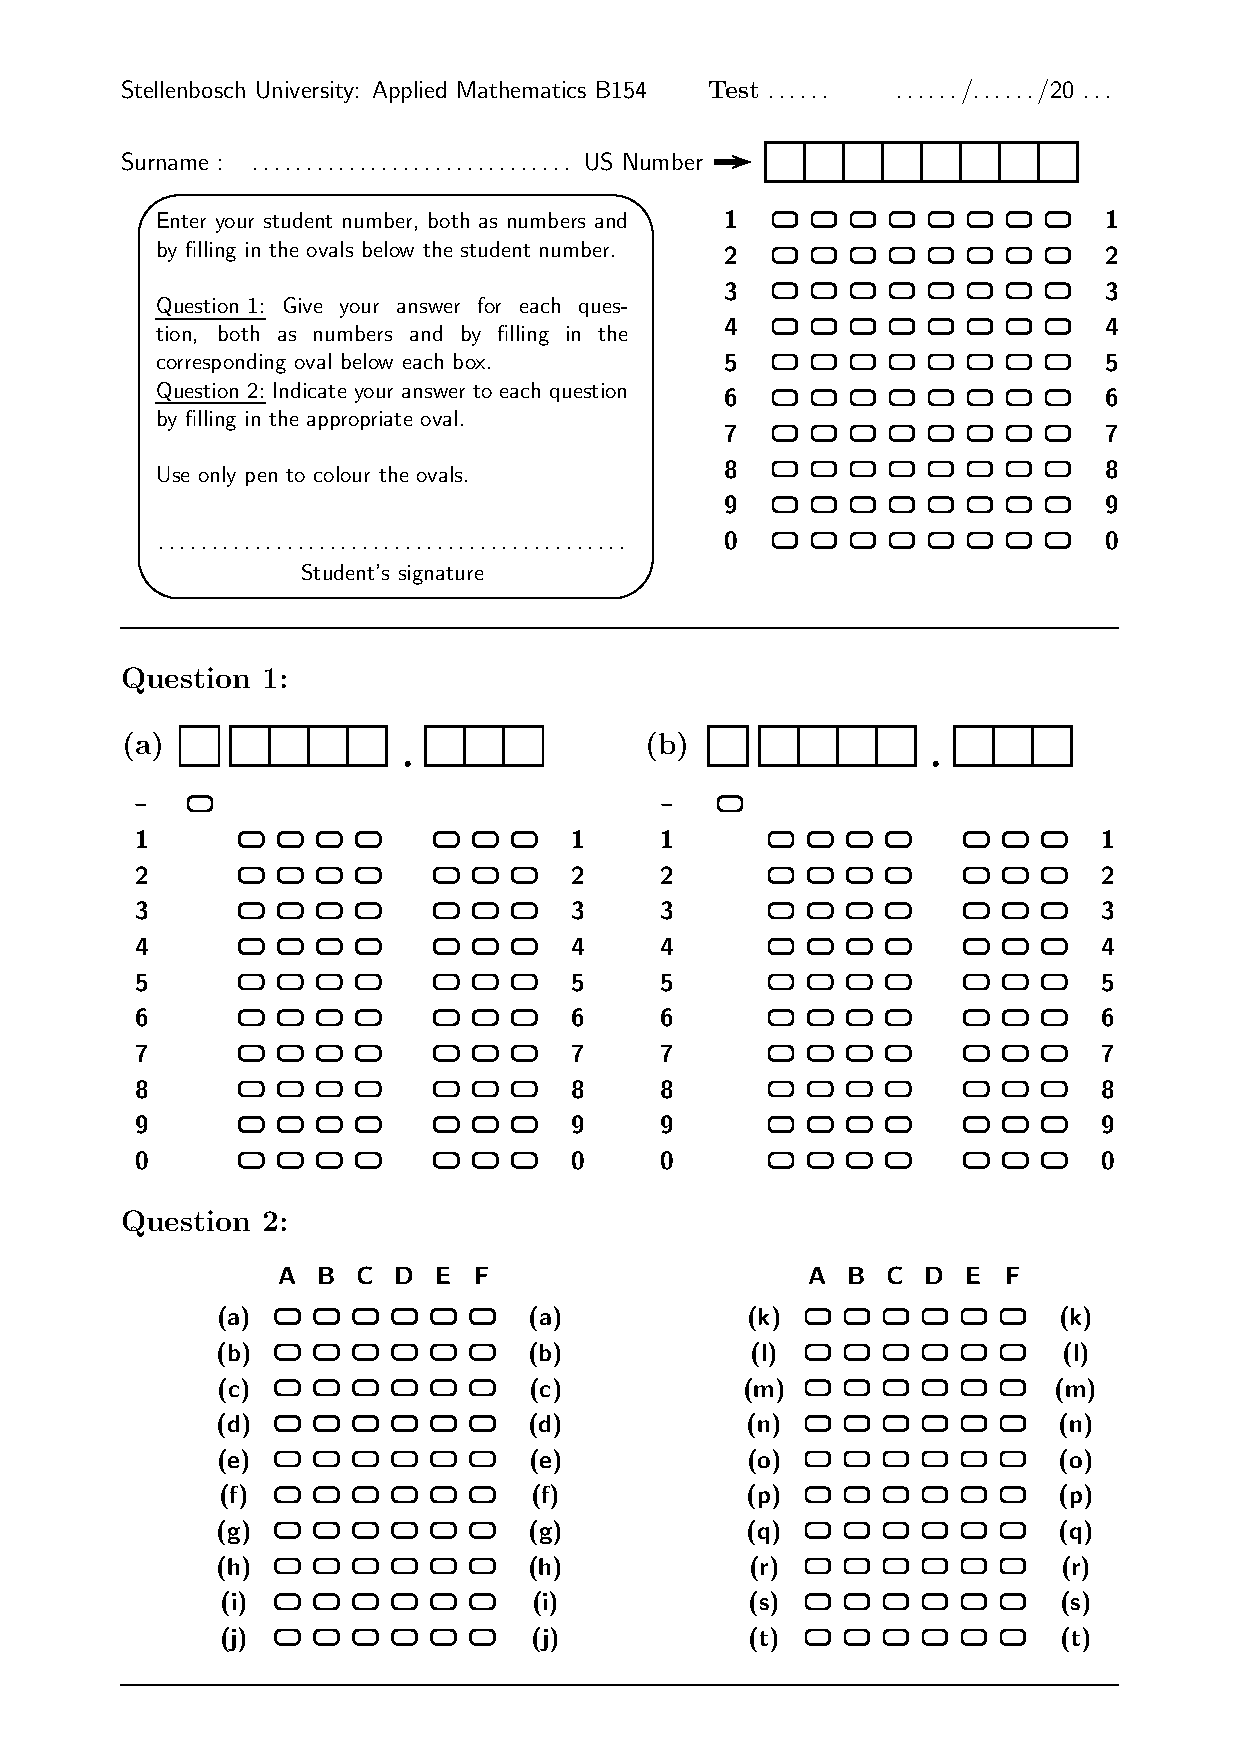
\includegraphics[width=12cm]{template2}\\
  \caption{Template allowing for numbered and multiple choice answers.}
  \label{fig:template2}
\end{figure}

\begin{figure}
  \centering
  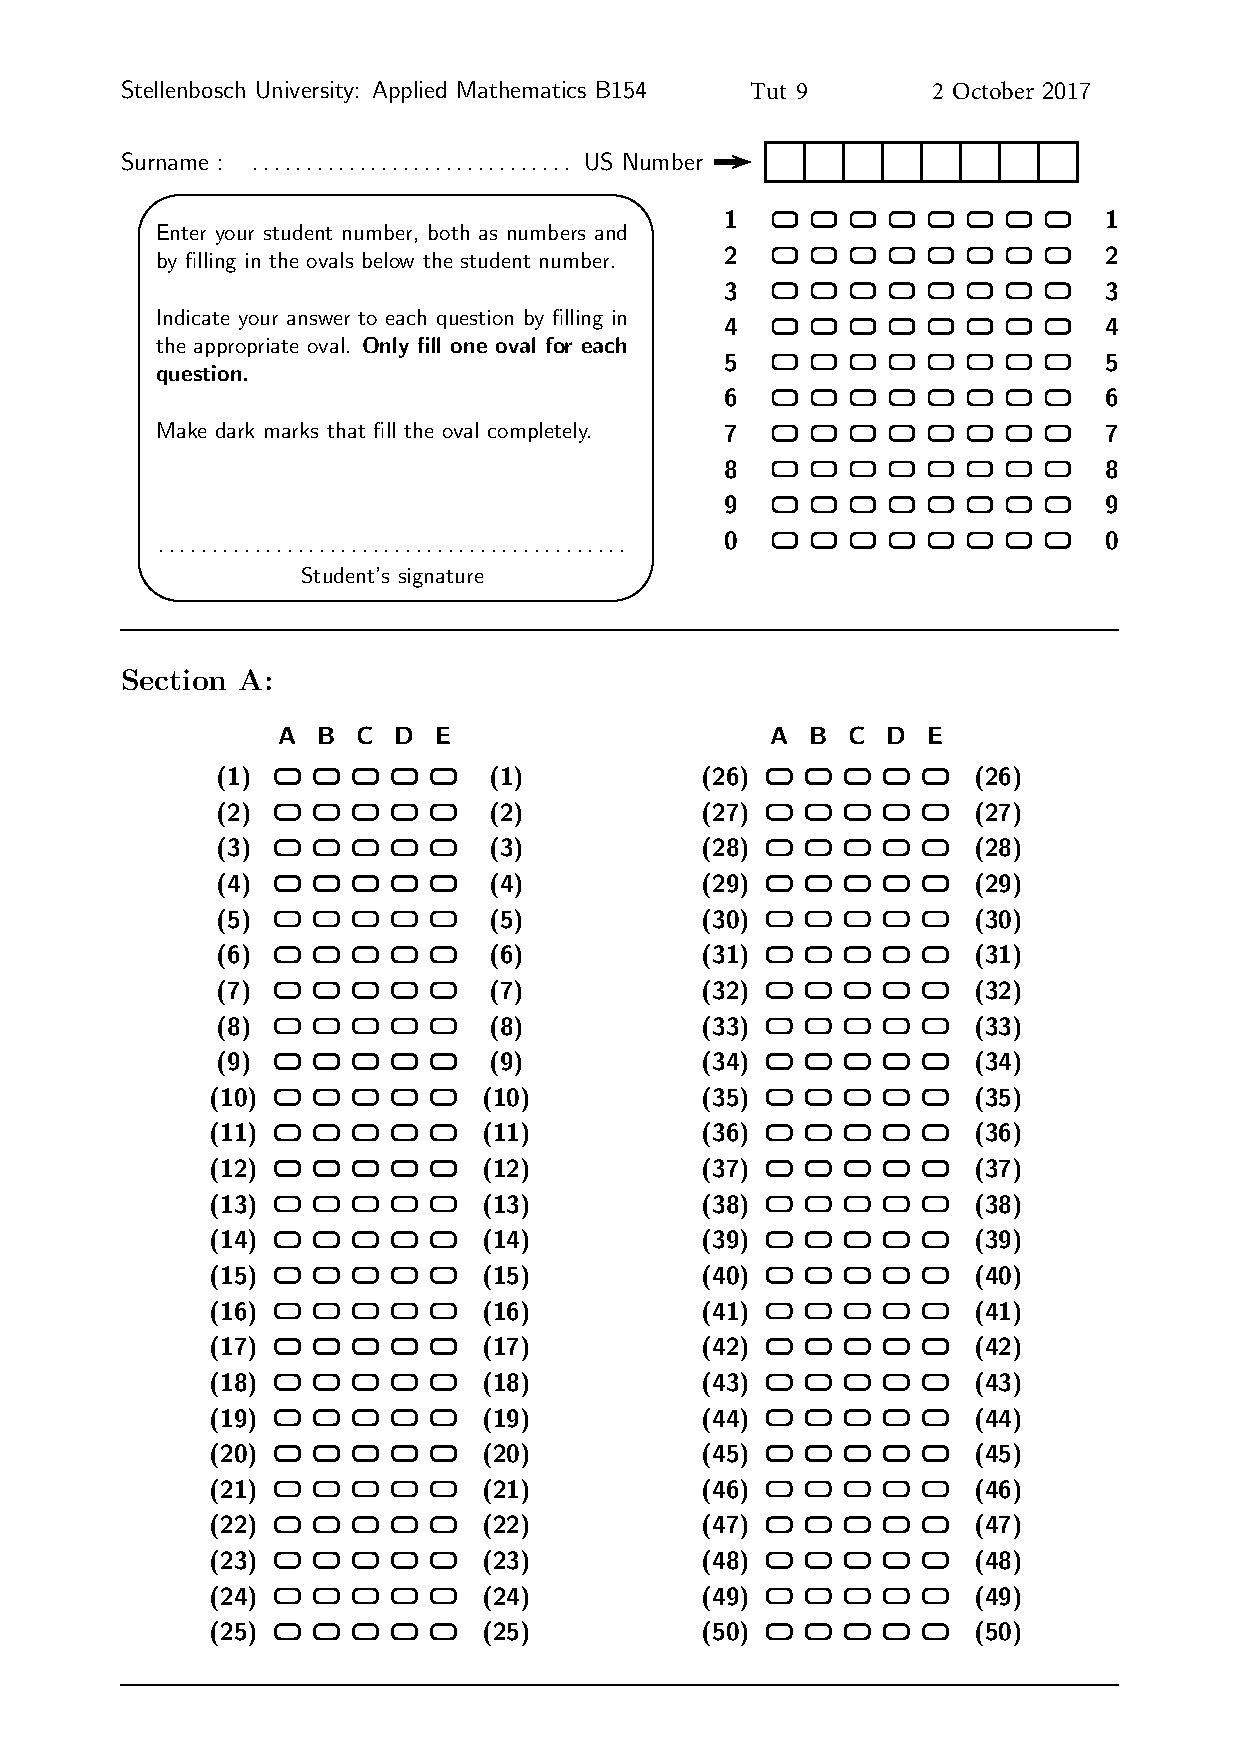
\includegraphics[width=12cm]{template3}\\
  \caption{Template focussed just on multiple choice type questions.}
  \label{fig:template3}
\end{figure}

\section{DCNN TensorFlow setup}
The DCNN structural setup diagram can be seen in Figure \ref{fig:DCNN}. This structure was directly used as constructed was constructed by the TensorFlow team.

\begin{figure}
  \centering
  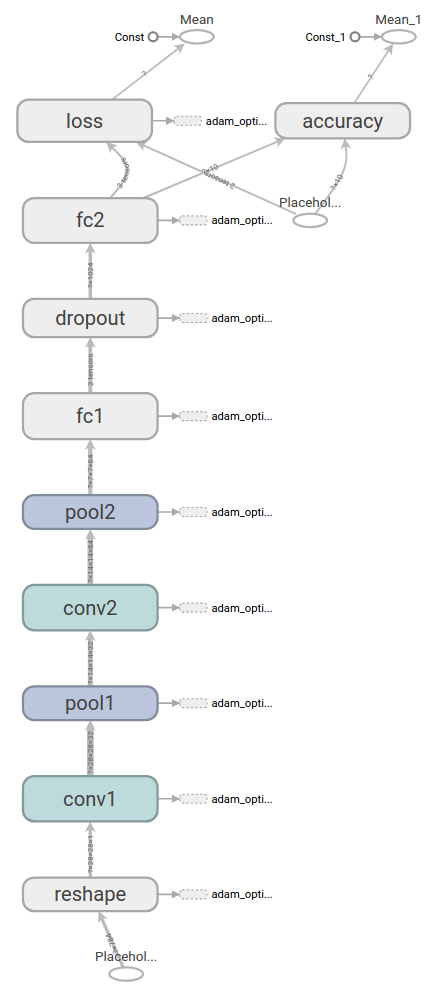
\includegraphics[width=7cm]{DCNN}\\
  \caption{DCNN structural setup diagram, from \citet{Tensor}}
  \label{fig:DCNN}
\end{figure} %BekkerMinutes


\end{document}


